\documentclass[11pt,a4paper,oneside,openany,indonesian]{report}
\usepackage[a4paper,top=25mm,bottom=25mm,left=30mm,right=25mm,headheight=16pt,headsep=7mm,footskip=12mm]{geometry}
\usepackage{iftex}
\ifLuaTeX
  \usepackage[bidi=basic,shorthands=off,provide=*]{babel}
\else
  \usepackage[bidi=default,shorthands=off,provide=*]{babel}
\fi
\ifPDFTeX\else\babelfont{rm}[]{Charter}\fi
\usepackage{hyperref}
% Shared preamble for the Jakarta TGA chapters.
\usepackage{xcolor}
\usepackage{graphicx}
\usepackage{amsmath,amssymb}
\usepackage{iftex}
\ifPDFTeX
  \usepackage[T1]{fontenc}
  \usepackage[utf8]{inputenc}
  \usepackage{textcomp}
\else
  \usepackage{unicode-math}
  \defaultfontfeatures{Scale=MatchLowercase}
  \defaultfontfeatures[\rmfamily]{Ligatures=TeX,Scale=1}
\fi
\usepackage{lmodern}
\ifPDFTeX\else
  \setmainfont[]{Times New Roman}
  \setsansfont[]{Arial}
  \IfFontExistsTF{Consolas}{\setmonofont[]{Consolas}}{\setmonofont[]{Courier New}}
\fi
\IfFileExists{microtype.sty}{\usepackage{microtype}}{}
\usepackage{longtable,booktabs,array,tabularx,adjustbox,calc}
\usepackage{pdflscape}
\usepackage{caption}
\captionsetup[table]{skip=6pt}
\newcounter{none}
\usepackage{float}
\usepackage{setspace}
\usepackage{ragged2e}
\usepackage{titlesec}
\usepackage{enumitem}
\usepackage{needspace}
\usepackage{fancyhdr}
\usepackage{newunicodechar}
\usepackage{bookmark}
\usepackage{xurl}
\usepackage{csquotes}
\usepackage[backend=biber,style=authoryear,maxcitenames=2,maxbibnames=99,uniquelist=false,uniquename=false]{biblatex}
\DeclareLanguageMapping{indonesian}{english}
\DefineBibliographyStrings{english}{and={dan},andothers={dkk\adddot}}
\DefineBibliographyStrings{indonesian}{and={dan},andothers={dkk\adddot}}
\AtBeginDocument{\renewcommand*{\finalnamedelim}{\addspace dan\space}}
\addbibresource{references.bib}
\DeclareFieldFormat{title}{#1}
\DeclareFieldFormat[article,inbook,incollection,inproceedings,inreference,patent,thesis,unpublished]{title}{#1}
\AtBeginBibliography{\small\setlength{\bibitemsep}{0.15em}}

\newunicodechar{∅}{\ensuremath{\varnothing}}

% Placeholder untuk gambar yang dibuat manual (peta GIS). Ganti dengan \includegraphics setelah berkas target tersedia.
\newcommand{\GambarPlaceholder}[2][7cm]{%
  \fbox{\parbox[c][#1][c]{0.92\linewidth}{\centering\small
    \textbf{PLACEHOLDER GAMBAR}\\[0.6em]#2}}}

\definecolor{Ink}{HTML}{222222}
\definecolor{RuleGray}{HTML}{666666}

\AtBeginDocument{%
  \hypersetup{linkcolor=Ink,citecolor=Ink,urlcolor=Ink,pdfborder={0 0 0}}%
  \urlstyle{same}%
}

\setstretch{1.5}
\setlength{\parindent}{1.1em}
\setlength{\parskip}{0.28em}
\setlength{\emergencystretch}{2.5em}
\clubpenalty=10000
\widowpenalty=10000
\displaywidowpenalty=10000
\raggedbottom

\setlist[itemize]{leftmargin=1.7em,itemsep=0.25em,topsep=0.35em}
\setlist[enumerate]{leftmargin=1.9em,itemsep=0.25em,topsep=0.35em}

\titleformat{\chapter}[display]
  {\normalfont\bfseries\centering\color{Ink}}
  {}{0pt}{\Large\hyphenpenalty=10000\exhyphenpenalty=10000}
\titlespacing*{\chapter}{0pt}{-6pt}{18pt}
\titleformat{\section}{\Needspace{4\baselineskip}\large\bfseries\color{Ink}}{\thesection}{0.7em}{}
\titleformat{\subsection}{\Needspace{3\baselineskip}\normalsize\bfseries\color{Ink}}{\thesubsection}{0.7em}{}
\titleformat{\subsubsection}{\Needspace{3\baselineskip}\normalsize\bfseries\color{Ink}}{\thesubsubsection}{0.7em}{}

\pagestyle{plain}
\fancyhf{}
\fancyfoot[C]{\thepage}
\renewcommand{\headrulewidth}{0pt}
\renewcommand{\footrulewidth}{0pt}
\fancypagestyle{plain}{%
  \fancyhf{}
  \fancyfoot[C]{\thepage}
  \renewcommand{\headrulewidth}{0pt}
}

\renewcommand{\arraystretch}{1.2}
\setlength{\extrarowheight}{1pt}
\setlength{\tabcolsep}{4pt}
\providecommand{\tightlist}{\setlength{\itemsep}{0pt}\setlength{\parskip}{0pt}}
\setlength{\LTpre}{0.5em}
\setlength{\LTpost}{0.8em}
\AtBeginEnvironment{longtable}{\footnotesize\setstretch{1.0}\setlength{\tabcolsep}{3pt}\setlength{\extrarowheight}{1pt}}
\AtBeginEnvironment{table}{\setstretch{1.0}}
\AtBeginEnvironment{figure}{\setstretch{1.0}}
\AtBeginEnvironment{quote}{\small\setlength{\leftskip}{1.2em}\setlength{\rightskip}{1.2em}}

\graphicspath{{figures/}}

\hypersetup{
  pdftitle={TGA PWK Jakarta - Bab 1--4},
  pdfauthor={Mahastri Laksita Sam Widita},
  pdflang={id-ID},
  hidelinks
}

\title{\textbf{Borrowed Size atau Agglomeration Shadow?}\\[0.4em]
Analisis Hubungan Integrasi Metropolitan dengan Kematangan Pusat-Pusat Sekunder di Kawasan Aglomerasi Jakarta}
\providecommand{\subtitle}[1]{\gdef\thesubtitle{#1}}
\subtitle{Naskah Bab 1--4}
\author{Mahastri Laksita Sam Widita\\NIM 22/503065/TK/54947\\[0.5em]
Pembimbing: Rendy Bayu Aditya\\[0.5em]
Program Studi Perencanaan Wilayah dan Kota\\
Departemen Teknik Arsitektur dan Perencanaan\\
Fakultas Teknik\\
Universitas Gadjah Mada}
\date{Kabupaten Sleman, Daerah Istimewa Yogyakarta\\2026}

\makeatletter
\renewcommand{\maketitle}{%
  \begin{titlepage}
    \centering
    {\Large\bfseries TUGAS AKHIR\par}
    \vfill
    {\LARGE\bfseries \@title\par}
    \vspace{1.2cm}
    {\large \thesubtitle\par}
    \vfill
    {\large \@author\par}
    \vfill
    {\large \@date\par}
  \end{titlepage}}
\makeatother

\begin{document}
\maketitle
\tableofcontents
\clearpage

\chapter{Pendahuluan}

\section{Latar belakang}

Perkembangan metropolitan Jakarta tidak berhenti pada batas administratif DKI Jakarta. Permukiman, kawasan industri, pusat pelayanan, dan jaringan transportasi berkembang di wilayah sekitarnya, sementara perjalanan penduduk dan kegiatan ekonomi menghubungkan berbagai bagian kawasan tersebut. Jakarta tetap menjadi pusat dominan, tetapi sejumlah kawasan di sekitarnya telah menjadi konsentrasi penduduk, pekerjaan, industri, dan pelayanan. Kajian mengenai Jabotabek dan Jabodetabek mencatat pergeseran kegiatan ke pinggiran, perkembangan kota baru dan kawasan industri, serta arus komuter antarpinggiran \parencite{henderson1996,hudalahfirman2012,hudalahetal2013,sadewoetal2023}.

Keberadaan beberapa konsentrasi di luar Jakarta belum menunjukkan sistem metropolitan yang seimbang. Polisentrisitas morfologis, yang terlihat dari persebaran konsentrasi penduduk atau pekerjaan, berbeda dari polisentrisitas fungsional yang terbentuk melalui arus dan interaksi antarpusat \parencite{burgermeijers2012}. Suatu kawasan dapat mempunyai banyak pusat secara fisik, tetapi hubungan fungsionalnya tetap terpusat, hierarkis, atau terfragmentasi. Hubungan yang kuat dengan Jakarta juga tidak selalu berarti ketergantungan sepihak. Pusat sekunder dapat menarik pekerja, melayani pasar yang lebih luas, atau berhubungan langsung dengan pusat sekunder lain. Analisis karena itu harus mempertahankan arah dan asimetri relasi, alih-alih mereduksinya sejak awal menjadi satu skor keterhubungan.

Persoalan berikutnya adalah apakah pertumbuhan pusat-pusat di sekitar Jakarta diikuti oleh penguatan fungsi lokal. Pertambahan penduduk, luas kawasan terbangun, fasilitas, atau pekerjaan menunjukkan dimensi perkembangan yang berbeda. Dekonsentrasi manufaktur, misalnya, dapat meningkatkan jumlah pekerjaan di pinggiran tanpa diikuti perpindahan fungsi keputusan, layanan bisnis, atau layanan berorde tinggi. Literatur mengenai spesialisasi fungsional menunjukkan bahwa produksi dapat tersebar ke kota yang lebih kecil ketika fungsi pengendalian dan layanan strategis tetap terkonsentrasi di kota besar \parencite{durantonpuga2005}. Dalam konteks Jabodetabek, pertumbuhan kawasan industri atau kota baru karena itu tidak cukup untuk menyimpulkan bahwa suatu pusat telah matang pada seluruh domain fungsi.

Perbedaan antara ukuran lokal dan fungsi aktual menjadi dasar konsep \emph{borrowed size}. Konsep ini menjelaskan kemungkinan bahwa kota atau pusat yang lebih kecil memperoleh fungsi atau kinerja yang biasanya diasosiasikan dengan kota lebih besar melalui relasinya dengan pusat lain. Namun, kedekatan geografis tidak cukup untuk membuktikan peminjaman ukuran. Relasi perlu ditunjukkan melalui arus atau interaksi, sedangkan fungsi aktual perlu dibandingkan dengan fungsi yang secara wajar diharapkan berdasarkan massa dan karakteristik lokal \parencite{meijersburger2017,meijersetal2016}. Surplus fungsi relatif yang tidak disertai bukti relasional belum dapat disebut \emph{borrowed size}.

Hubungan dengan pusat dominan juga dapat berkaitan dengan hasil yang kurang menguntungkan. Kompetisi atas tenaga kerja, permintaan, investasi, dan fungsi berorde tinggi dapat membuat pusat sekunder tetap berada di bawah tingkat fungsi yang diharapkan. Pola tersebut sering dibahas melalui konsep \emph{agglomeration shadow}. Meskipun demikian, bukti empiris tidak menunjukkan satu tanda hubungan yang berlaku umum. Manfaat jaringan, defisit fungsi, dan hasil campuran berubah menurut ukuran pusat, sektor, posisi jaringan, hierarki, dan skala analisis \parencite{volgmannrusche2020,yangzhudu2022,zhenshilu2023}. Temuan tandingan juga menunjukkan bahwa kedekatan dengan kota besar dapat berkaitan dengan pertumbuhan wilayah sekitarnya, sehingga \emph{shadow} tidak boleh diasumsikan sebelum analisis dilakukan \parencite{partridgeetal2009,sunding2016}.

Perbedaan hasil antardomain sangat mungkin muncul di Jabodetabek. Sebuah pusat dapat mempunyai surplus pekerjaan manufaktur sekaligus defisit layanan tingkat tinggi. Penduduknya mungkin memperoleh akses ke pasar kerja metropolitan sambil menanggung waktu dan biaya perjalanan yang besar. Pekerjaan yang berada di suatu pusat pun belum tentu dinikmati oleh penduduk setempat. Kajian komuter dan akses pekerjaan di Jakarta menunjukkan bahwa manfaat akses, penggunaan aktual, persaingan antarpencari kerja, dan beban perjalanan adalah objek yang berbeda \parencite{andani2021,aritenang2022,andani2025}. Manfaat, beban, dan ketergantungan karena itu tidak dilebur menjadi satu skor bersih. Analisis harus tetap menunjukkan penerima manfaat dan penanggung beban.

Literatur internasional membahas fungsi pinjaman, kinerja pinjaman, dan \emph{agglomeration shadow}. Penelitian Jabodetabek telah menguraikan dekonsentrasi industri, perkembangan kota baru, perubahan struktur metropolitan, komuter, akses pekerjaan, dan fragmentasi tata kelola. Dalam korpus yang ditelusuri, pembahasan tersebut belum dirangkai dalam satu pengukuran yang mempertahankan arah relasi metropolitan, membandingkan fungsi aktual per domain dengan ekspektasi dari massa lokal, memisahkan manfaat dari beban menurut aktor dan lokasi, serta menguji ketahanan hasil terhadap keputusan analitis. Pernyataan ini hanya berlaku pada korpus yang diperiksa; ia tidak menyatakan bahwa susunan penelitian serupa belum pernah dibuat.

Penelitian ini tidak memilih \emph{borrowed size} atau \emph{agglomeration shadow} sebagai jawaban awal. Kedua konsep dipakai untuk menafsirkan konfigurasi observasional setelah relasi metropolitan, fungsi relatif, dan penjelasan alternatif diperiksa. Objek yang diestimasi adalah hubungan antara relasi metropolitan terarah suatu pusat sekunder dan deviasi fungsi aktual dari fungsi yang diharapkan menurut massa serta karakteristik lokal. Pengukuran dilakukan per domain agar surplus pada satu domain tidak menutupi defisit pada domain lain.

Penelitian ini berfokus pada pusat-pusat sekunder di Kawasan Aglomerasi Jakarta. DKI Jakarta diperlakukan sebagai satu inti pada spesifikasi utama untuk membaca hubungan eksternal dan tanggung jawab administratif, tetapi kemungkinan bahwa arus menuju subpusat yang berbeda di dalam DKI akan diperiksa sebagai spesifikasi alternatif. Batas administratif tetap dipertahankan sebagai batas kewenangan, pelayanan, dan tanggung jawab pemerintah. Jejak fungsional yang melintasi batas dibaca sebagai hubungan metropolitan, bukan sebagai perluasan yurisdiksi Jakarta.

Penelitian ini tidak mengajukan konsep baru dan tidak menganggap integrasi selalu menguntungkan atau merugikan. Sumbangan penelitian terletak pada penyatuan lima operasi: mengukur relasi terarah, membentuk tolok ukur fungsi dari massa lokal, menganalisis hubungan per domain, memisahkan manfaat dari beban, dan memeriksa ketahanan hasil. Tipologi hanya menjadi ringkasan akhir jika profil kontinu dan ketidakpastiannya telah diperiksa.

Pemilihan data merupakan bagian dari rancangan pengukuran. Penelitian ini menggunakan proksi dan sumber terbuka untuk membentuk informasi lokasi, fungsi, dan hubungan metropolitan. Sumber administratif terbuka, peta kolaboratif, direktori usaha dan fasilitas, informasi transportasi, serta penginderaan jauh dinilai dari kesesuaiannya dengan pertanyaan penelitian. Sumber alternatif dapat lebih tepat daripada data agregat yang tersedia, tetapi keunggulan itu harus dibuktikan untuk setiap konstruk, wilayah, dan periode.

\begin{figure}[H]
  \centering
  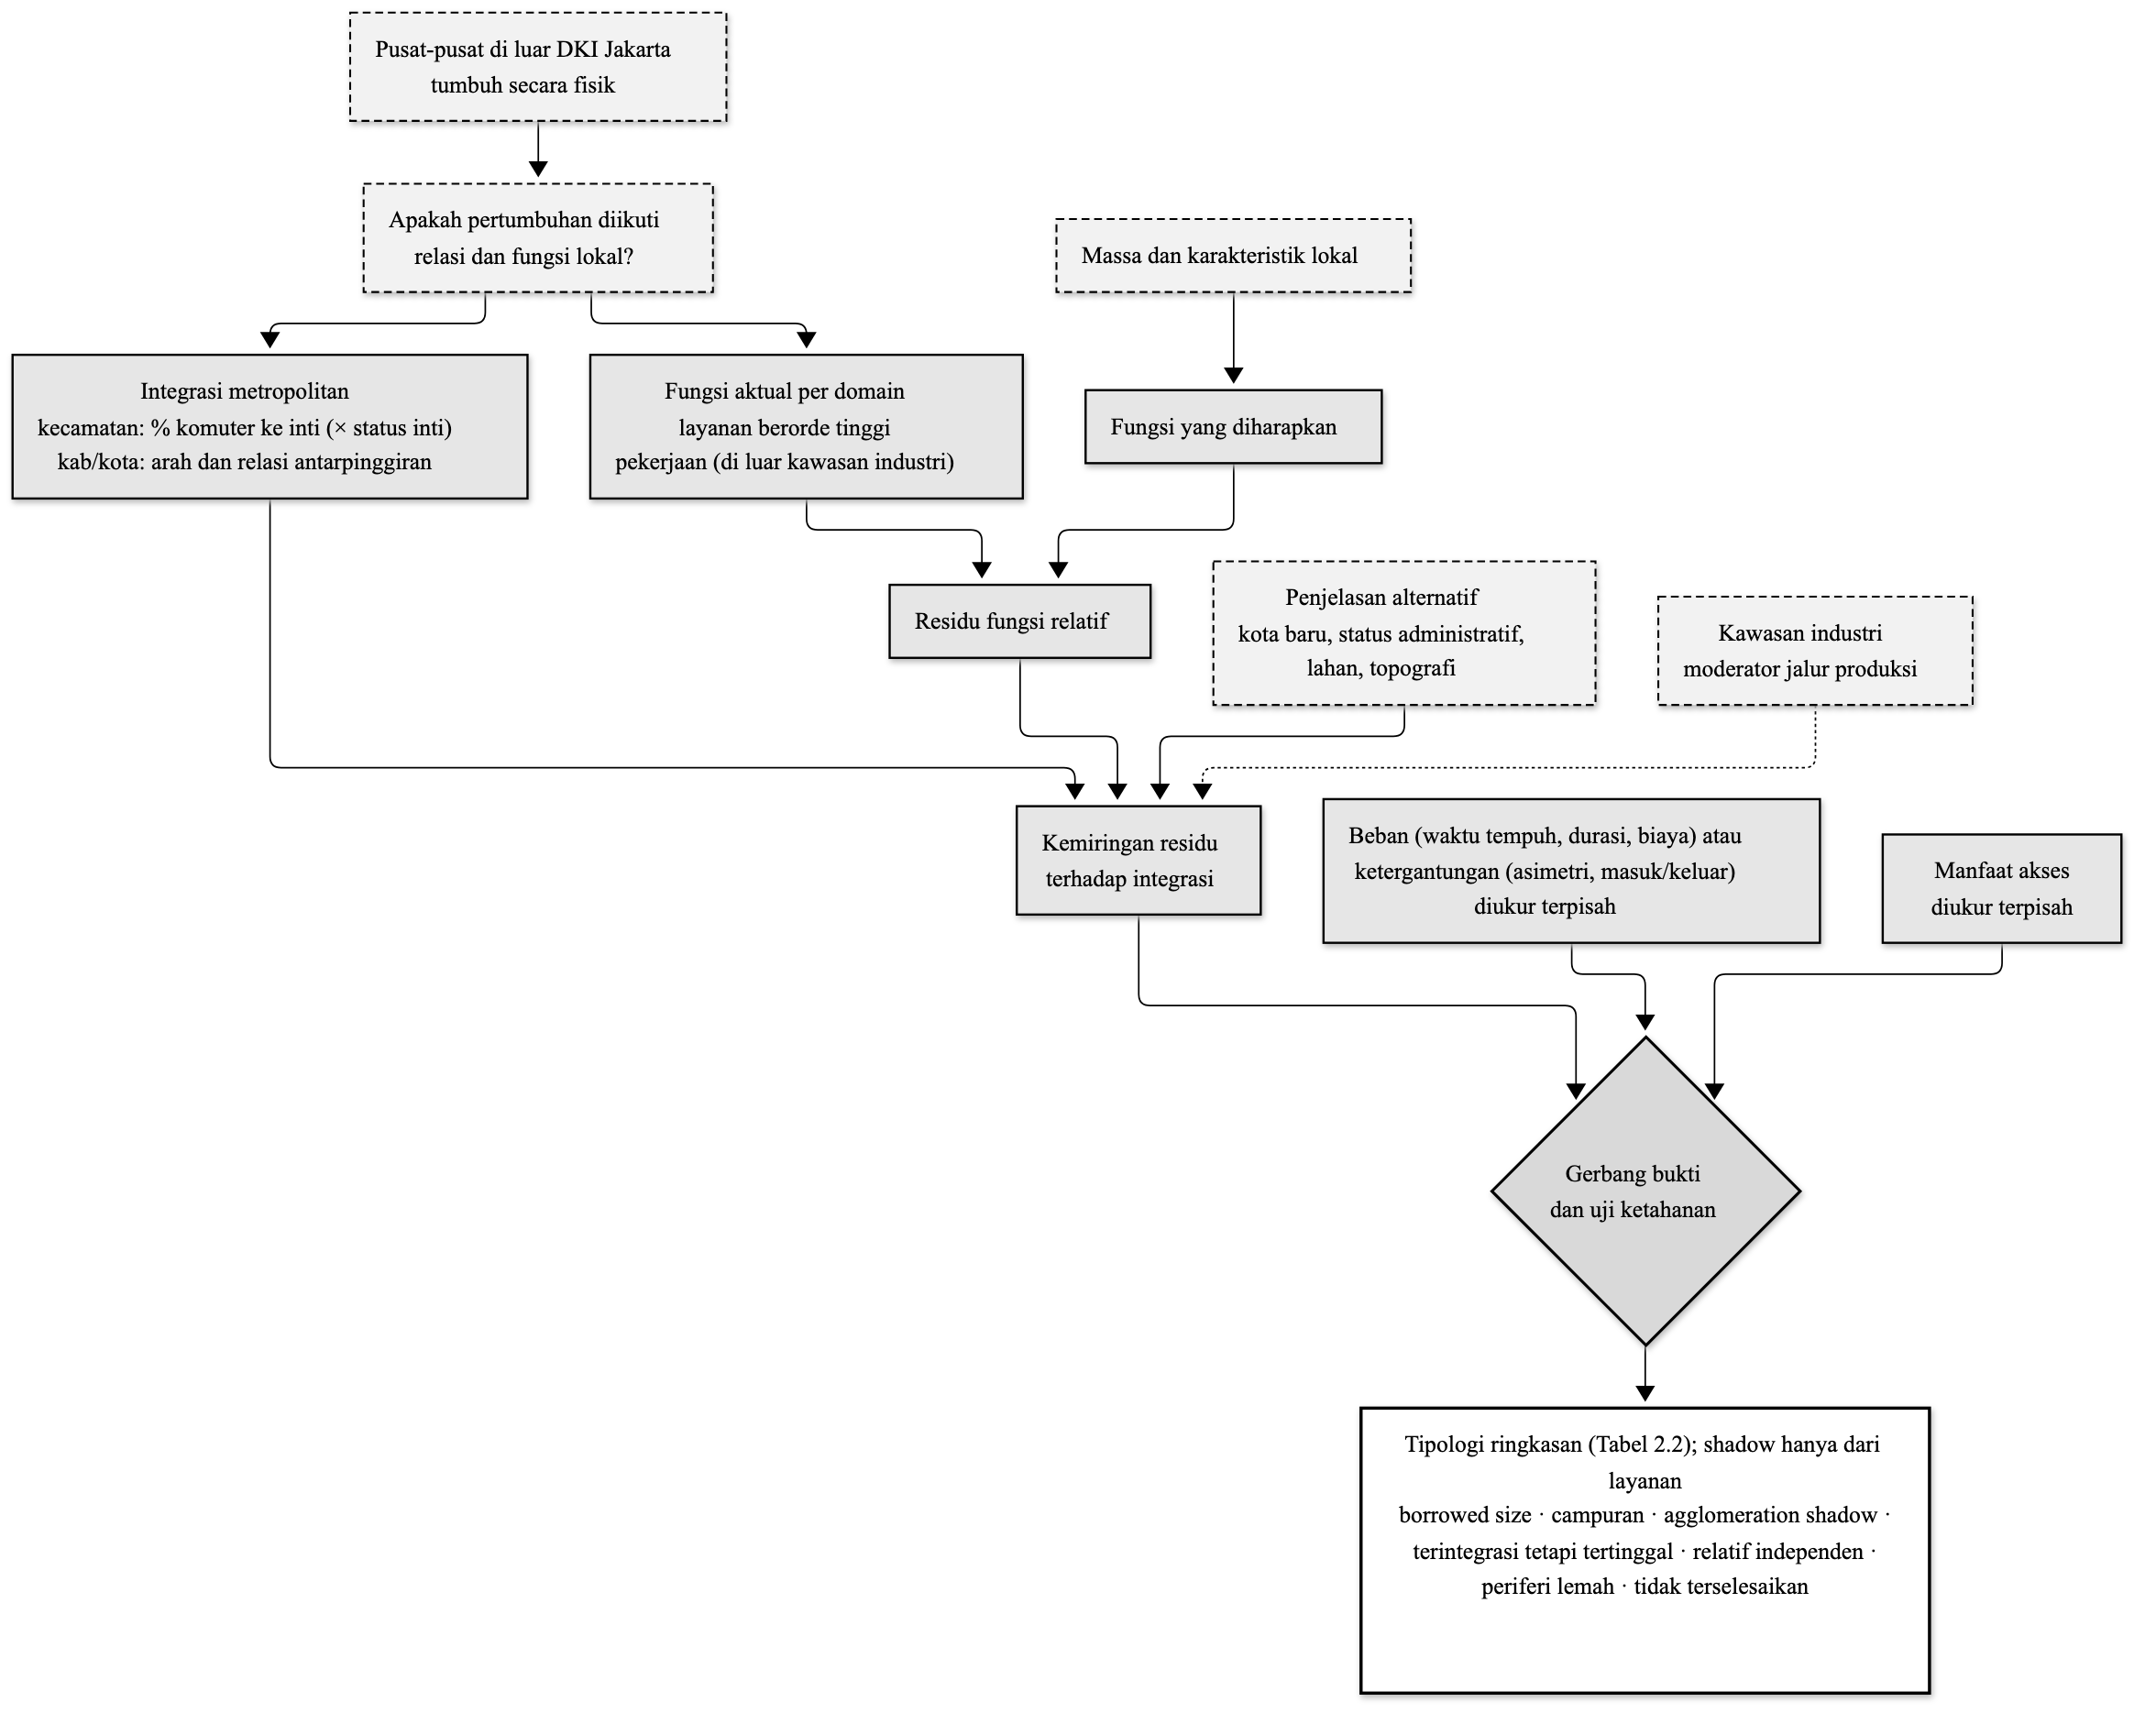
\includegraphics[width=\textwidth]{figures/bab1_logika_penelitian.png}
  \caption{Logika masalah dan objek pengukuran penelitian. Diagram merangkum hubungan antara perkembangan pusat di luar DKI Jakarta, relasi metropolitan terarah, fungsi relatif, beban, dan gerbang interpretasi.}
  \label{fig:bab1-logika}
\end{figure}

\section{Rumusan masalah}

Transformasi metropolitan Jakarta telah membentuk pusat kegiatan di luar inti administratif. Keberadaan pusat tersebut belum menjelaskan kualitas relasinya dengan Jakarta ataupun kekuatan fungsi lokalnya. Hubungan metropolitan dapat berkaitan dengan surplus fungsi pada satu domain, defisit pada domain lain, manfaat akses, beban perjalanan, atau ketergantungan yang asimetris. Masalah penelitian terletak pada konfigurasi hubungan dan fungsi relatif yang teramati pada setiap pusat.

Masalah tersebut dirumuskan dalam tiga pertanyaan penelitian:

\begin{enumerate}
  \item Bagaimana arah, intensitas, dan asimetri relasi pusat-pusat sekunder dengan Jakarta serta dengan pusat sekunder lain berdasarkan pengamatan dan estimasi dari sumber terbuka?
  \item Bagaimana fungsi relatif, manfaat, dan beban pada setiap pusat sekunder dan domain yang diteliti, serta bagaimana nilainya berubah pada indikator yang memiliki seri sebanding?
  \item Bagaimana integrasi metropolitan berhubungan dengan fungsi relatif pusat-pusat sekunder setelah kondisi lokal dan penjelasan alternatif diperiksa, serta konfigurasi apa yang konsisten dengan \textit{borrowed size}, \textit{agglomeration shadow}, hasil campuran, atau hasil yang belum terselesaikan?
\end{enumerate}

Analisis sensitivitas tidak menjadi pertanyaan substantif tersendiri. Analisis tersebut digunakan untuk menilai ketahanan jawaban atas ketiga pertanyaan melalui perubahan unit, delineasi, indikator, transformasi, tolok ukur, bobot, ambang, dan spesifikasi yang masih mengestimasi objek sejenis. Perubahan sumber atau konstruk yang menghasilkan estimand berbeda dilaporkan sebagai triangulasi atau perubahan estimand, bukan sebagai sensitivitas model yang ekuivalen.

\section{Tujuan penelitian}

Tujuan umum penelitian ini adalah menganalisis hubungan antara integrasi metropolitan dan fungsi relatif pusat-pusat sekunder di Kawasan Aglomerasi Jakarta dengan membedakan domain fungsi, manfaat, beban, dan ketahanan hasil terhadap keputusan analitis.

Tujuan khusus penelitian adalah:

\begin{enumerate}
  \item Mengukur dan memetakan arah, intensitas, serta asimetri relasi pusat-pusat sekunder dengan Jakarta dan dengan pusat sekunder lain berdasarkan pengamatan dan estimasi dari sumber terbuka.
  \item Mengukur atau mengestimasi fungsi relatif, manfaat, dan beban pada setiap pusat sekunder dan domain yang diteliti, serta membaca perubahannya pada indikator yang memiliki seri sebanding.
  \item Menganalisis hubungan integrasi metropolitan dengan fungsi relatif setelah kondisi lokal dan penjelasan alternatif diperiksa, lalu mengidentifikasi konfigurasi yang konsisten dengan \textit{borrowed size}, \textit{agglomeration shadow}, hasil campuran, atau hasil yang belum terselesaikan.
\end{enumerate}

\section{Batasan penelitian}

Penelitian ini dibatasi pada sistem Jabodetabek administratif yang mencakup DKI Jakarta, Kabupaten Bogor, Kota Bogor, Kota Depok, Kabupaten Tangerang, Kota Tangerang, Kota Tangerang Selatan, Kabupaten Bekasi, dan Kota Bekasi. Batas tersebut digunakan sebagai ruang kerja utama dan tidak menyatakan bahwa batas administratif identik dengan batas fungsional metropolitan. Tolok ukur utama dibentuk secara internal dari pusat-pusat sekunder Jabodetabek yang memiliki unit, periode, dan konstruk sebanding; DKI Jakarta tidak dimasukkan ke dalam pembentukan ekspektasi karena kedudukannya sebagai inti. Hasil fungsi relatif karena itu dibaca terhadap kawasan studi. Wilayah di luar cakupan hanya dapat digunakan sebagai pemeriksaan sensitivitas apabila keterbandingannya terbukti dan bukan syarat terlaksananya penelitian.

Unit substantif penelitian adalah kandidat pusat sekunder beserta wilayah tangkapan fungsionalnya. Unit perhitungan dapat berupa kecamatan, beberapa unit yang bersebelahan, zona asal-tujuan, titik fasilitas, atau sel raster sesuai resolusi sumber yang dapat dipertanggungjawabkan. Nilai kabupaten/kota tidak diturunkan ke kecamatan atau titik tanpa model eksplisit, asumsi yang terlihat, pemeriksaan independen, dan pelabelan sebagai estimasi.

Penelitian bertumpu pada proksi dan sumber terbuka. Data pemerintah terbuka dapat digunakan apabila sesuai, sedangkan data tertutup, permohonan kelembagaan, sensus usaha lengkap, data ponsel individu, atau matriks OD mikro bukan syarat rancangan. Ketersediaan koordinat, panjang seri, dan banyaknya sumber tidak otomatis membuktikan mutu pengukuran. Setiap proksi dinilai berdasarkan kesesuaian konstruk, cakupan spasial dan temporal, keterulangan, biaya pemerolehan, lisensi, dan hasil pemeriksaan independen.

Desain waktu bersifat multitemporal sesuai bukti. Perubahan hanya dianalisis pada indikator yang memiliki seri sebanding; indikator lain digunakan pada periode yang tersedia dengan tahun observasi yang ditulis jelas. Perubahan keterlihatan digital, perubahan kategori, dan perubahan batas tidak boleh diperlakukan otomatis sebagai perubahan fenomena. Panel lengkap dengan satu tahun jangkar untuk seluruh sumber tidak diasumsikan.

Analisis inti menggunakan paling banyak dua domain fungsi yang memiliki pengukuran atau proksi paling dapat dipertanggungjawabkan, dengan pekerjaan sebagai domain utama dan layanan berorde tinggi sebagai domain kedua apabila lolos audit. Domain lain hanya menjadi konteks atau pemeriksaan tambahan. Istilah kematangan dalam penelitian ini berarti kematangan fungsi lokal pada domain tersebut, bukan kesejahteraan penduduk, mutu pelayanan secara menyeluruh, ketahanan ekonomi, atau keberhasilan pembangunan. Jumlah titik usaha tidak disebut produktivitas, pendapatan, inovasi, atau kesejahteraan tanpa pengukuran atau model yang sesuai.

Rantai analisis minimum terdiri atas satu periode yang kompatibel, satu bukti relasi komuter terarah, satu domain fungsi yang dibentuk secara independen, tolok ukur internal, serta pembacaan surplus atau defisit relatif. Pengamatan multitemporal, domain kedua, CCTV, SUMO, dan Web GIS merupakan penguatan setelah rantai tersebut berjalan. Rekaman CCTV dapat diolah dengan deteksi YOLO dan pelacakan objek setelah cakupan, privasi, sudut pandang, dan galat hitung diperiksa. Hitungan CCTV tidak menjadi pengganti matriks asal-tujuan, sedangkan SUMO hanya digunakan jika kebutuhan kalibrasinya terpenuhi.

Hasil penelitian bersifat observasional dan asosiasional. Penelitian ini tidak mengidentifikasi pengaruh kausal Jakarta terhadap pusat sekunder, tidak menetapkan satu radius metropolitan yang benar, tidak menjamin bahwa setiap pusat akan masuk tipologi tertentu, dan tidak memprediksi dampak kebijakan masa depan. Istilah \emph{borrowed size} atau \emph{agglomeration shadow} digunakan sebagai interpretasi bersyarat setelah bukti relasional, fungsi relatif, penjelasan alternatif, dan ketahanan hasil diperiksa.

\section{Metode penelitian}

Penelitian ini memakai pendekatan kuantitatif, analisis spasial-relasional, dan desain studi kasus di Kawasan Aglomerasi Jakarta. Dimensi waktu mengikuti bukti yang tersedia. Perubahan hanya dihitung pada indikator dengan definisi, unit, dan cakupan yang sebanding; indikator lain dibaca pada periodenya masing-masing. Tahun dasar ditetapkan per modul setelah audit. Penelitian tidak mengasumsikan panel lengkap atau satu tahun jangkar untuk semua sumber. Hasilnya berupa pola, asosiasi, dan perubahan terukur, bukan bukti kausal.

Proksi dan sumber terbuka menjadi dasar pengukuran. Data pemerintah terbuka tetap digunakan ketika sesuai. Setiap sumber dinilai dari kesesuaian konstruk, cakupan ruang dan waktu, keterulangan pengolahan, serta biaya pemerolehan. Status resmi tidak otomatis menunjukkan mutu yang lebih tinggi. Unit substantifnya adalah pusat sekunder dan wilayah tangkapan analitis, sedangkan unit perhitungan mengikuti resolusi sumber. Data titik, bangunan, jaringan, dan raster dipertahankan pada resolusi asal. Data agregat hanya dialokasikan ke unit lebih rinci melalui model yang menjelaskan asumsi dan ketidakpastian; keluarannya disebut estimasi.

Analisis dimulai dengan menetapkan kandidat pusat sebelum fungsi relatif diketahui. Relasi utama berasal dari pasangan arus komuter yang diamati pada unit yang kompatibel. Dari satu matriks tersebut dihitung intensitas arus, orientasi menuju DKI, arus antarpusat sekunder, daya tarik masuk, \emph{self-containment}, dan asimetri sejauh definisi sumber mendukung. Aksesibilitas dari jaringan atau waktu tempuh dipisahkan dari arus aktual. Jika pasangan arus harus diestimasi, hasilnya hanya menjadi relasi utama setelah diperiksa terhadap bukti independen; jika syarat ini gagal, keluaran tersebut dibatasi sebagai eksplorasi. Rute, frekuensi, armada, kapasitas, dan penumpang tidak dipertukarkan maknanya.

Fungsi aktual diukur pada satu atau paling banyak dua domain inti. Domain pekerjaan dipasangkan dengan relasi komuter apabila arusnya diamati secara independen. Layanan berorde tinggi dapat menjadi domain kedua jika lokasi, kelas, kapasitas, atau akreditasinya dapat diperiksa dan indikator tersebut tidak digunakan untuk membentuk relasi. Pada setiap domain, fungsi aktual dibandingkan dengan fungsi yang diharapkan dari massa dan karakteristik lokal menggunakan pembanding internal Jabodetabek sebelum hubungan dengan integrasi diuji.

Tahap berikutnya menguji asosiasi antara relasi terarah dan residu fungsi pada domain yang memenuhi syarat independensi. Indikator yang membentuk relasi tidak dipakai kembali sebagai fungsi yang hendak dijelaskan. Jika OD sintetis menggunakan pekerjaan sebagai massa tujuan, pasangan tersebut tidak digunakan untuk menguji residu pekerjaan. Ketidakpastian diteruskan ke perhitungan, sedangkan jumlah parameter mengikuti jumlah pusat efektif. Jika jumlah pusat tidak memadai untuk regresi, analisis dibatasi pada profil dan perbandingan kelompok dengan batas interpretasi yang jelas.

\section{Manfaat penelitian}

\subsection{Manfaat teoretis}

Secara teoretis, penelitian ini memperjelas penggunaan \emph{borrowed size} dan \emph{agglomeration shadow} dalam sistem metropolitan yang hierarkis. Penelitian memisahkan massa lokal dari fungsi aktual, kedekatan dari relasi yang terealisasi, serta kematangan fungsi lokal dari akses, kinerja, dan kesejahteraan. Analisis dibatasi pada domain inti yang lolos audit agar perbedaan antardomain tetap terlihat tanpa memperluas objek penelitian.

\subsection{Manfaat metodologis}

Secara metodologis, penelitian ini menyediakan alur yang dapat diaudit dari delineasi pusat sampai pengukuran relasi, tolok ukur fungsi, residu per domain, manfaat dan beban menurut aktor, serta ketidakpastian hasil. Pemisahan peran indikator mengurangi hubungan matematis semu. Sensitivitas, triangulasi, dan perubahan estimand juga dibedakan agar perbandingan objek yang berbeda tidak disebut sebagai bukti ketahanan.

\subsection{Manfaat praktis}

Secara praktis, penelitian ini memberi gambaran yang lebih terpilah mengenai posisi pusat sekunder kepada pemerintah daerah dan lembaga koordinasi metropolitan. Profil relasi, fungsi relatif, manfaat, dan beban dapat membedakan kebutuhan penguatan fungsi lokal, hubungan antarpusat, pengurangan beban perjalanan, atau koordinasi lintas batas. Keluaran ini bersifat diagnostik. Penelitian tidak menetapkan perubahan batas administrasi, memilih satu bentuk kelembagaan, atau memprediksi dampak kebijakan tanpa analisis tambahan.

\section{Struktur penulisan}

Penelitian ini disusun dalam enam bab. Bab 1 menjelaskan latar belakang, rumusan masalah, tujuan, batasan, ringkasan metode, manfaat, dan struktur penulisan. Bab 2 membangun konsep kunci, menyintesis perdebatan penelitian terdahulu, dan menyusun kerangka teori serta kerangka konseptual yang menghubungkan massa lokal, relasi metropolitan, fungsi relatif, manfaat, beban, dan diagnosis bersyarat.

Bab 3 menjelaskan pendekatan dan desain penelitian, ruang lingkup, unit amatan dan unit analisis, pengumpulan data, serta tahapan analisis. Bab 4 menggambarkan Kawasan Aglomerasi Jakarta sejauh diperlukan untuk memahami struktur wilayah, kandidat pusat sekunder, hubungan administratif, dan konteks fungsi metropolitan. Bab 5 menyajikan serta membahas hasil menurut pertanyaan penelitian. Bab 6 merangkum jawaban penelitian, batas inferensi, dan rekomendasi yang sesuai dengan temuan.

\clearpage

\chapter{Kajian Pustaka}

\section{Penjelasan konsep-konsep kunci}

Konsep dalam bab ini dipakai untuk membedakan objek yang sering tercampur dalam pembahasan metropolitan. Ukuran lokal, fungsi, kinerja, aksesibilitas, konektivitas, dan integrasi fungsional bukan sinonim. Sebuah pusat sekunder dapat mempunyai penduduk besar, akses yang baik, dan arus keluar yang kuat pada saat yang sama. Susunan seperti itu belum cukup untuk disebut peminjaman ukuran atau bayangan aglomerasi.

\subsection{Ekonomi aglomerasi dan disekonomi aglomerasi}

Ekonomi aglomerasi adalah manfaat yang muncul ketika rumah tangga dan perusahaan berdekatan dengan banyak orang, pekerja, pemasok, pengetahuan, infrastruktur, dan amenitas. Mekanisme yang sering digunakan untuk menjelaskannya ialah berbagi, mencocokkan, dan belajar: berbagi fasilitas atau input, mencocokkan kebutuhan perusahaan dengan tenaga kerja, serta memperoleh pembelajaran dan pengetahuan dari interaksi yang berulang \parencite{durantonpuga2004}. Konsentrasi juga menimbulkan biaya, seperti kemacetan, harga lahan, polusi, tekanan jaringan, dan kompetisi atas sumber daya. Karena manfaat dan biaya bergerak bersama dengan cara yang berbeda, aglomerasi tidak boleh diperlakukan sebagai keuntungan yang selalu positif.

Dalam penelitian ini, teori aglomerasi menjadi garis dasar untuk membaca hubungan ukuran dan fungsi. Jika pusat yang lebih besar cenderung menopang lebih banyak fungsi, maka fungsi pusat kecil yang melebihi ekspektasi ukurannya perlu dijelaskan melalui relasi lain, karakteristik khusus, atau kesalahan pengukuran. Kenaikan kepadatan juga tidak langsung berarti kenaikan produktivitas; arah hubungan dapat berubah menurut sektor, skala, kelompok sosial, dan kondisi wilayah.

\subsection{Ukuran lokal, fungsi metropolitan, dan kinerja}

Tiga objek dipisahkan sejak awal. Ukuran lokal adalah massa yang dimiliki unit, misalnya penduduk, tenaga kerja, jumlah usaha, luas terbangun, atau kepadatan. Fungsi metropolitan adalah kemampuan menyediakan kegiatan atau layanan yang melampaui kebutuhan rutin unit, seperti pekerjaan khusus, layanan kesehatan dan pendidikan berorde tinggi, layanan bisnis, fungsi budaya, atau pusat kegiatan. Kinerja adalah hasil yang dicapai, misalnya produktivitas, pendapatan, inovasi, atau kesejahteraan.

Satu pusat dapat besar secara demografis tetapi terbatas pada fungsi keputusan. Sebaliknya, pusat yang lebih kecil dapat mempunyai layanan yang lebih beragam daripada yang lazim bagi ukurannya. Jumlah fasilitas, pekerjaan, PDRB, dan kinerja kesejahteraan karena itu tidak boleh saling menggantikan tanpa penjelasan konstruk, satuan, dan batas interpretasi.

\subsection{Sistem perkotaan, hierarki pusat, dan pusat sekunder}

Sistem perkotaan merupakan himpunan pusat yang saling berhubungan melalui arus manusia, barang, jasa, modal, informasi, dan pembagian fungsi. Teori tempat sentral membantu menjelaskan mengapa layanan berorde tinggi memerlukan ambang permintaan dan jangkauan pasar yang lebih besar. Pandangan jaringan melengkapi penjelasan tersebut dengan menunjukkan bahwa fungsi sebuah pusat juga ditentukan oleh posisinya terhadap pusat lain dan oleh kualitas relasi di antara pusat-pusat tersebut \parencite{burgermeijers2016}.

Dalam penelitian ini, \textit{pusat sekunder} berarti pusat di luar inti Jakarta yang memiliki konsentrasi penduduk, pekerjaan, layanan, atau aktivitas serta berpotensi menjalankan fungsi subregional atau metropolitan. Status tersebut tidak ditentukan hanya oleh label kota administratif atau kedekatan dengan Jakarta. Kandidat pusat akan diperoleh dari bukti spasial dan fungsi yang tersedia, lalu diperiksa kembali terhadap ukuran unit dan periode pengamatan.

\subsection{Polisentrisitas morfologis dan fungsional}

Polisentrisitas morfologis menunjuk pada keberadaan beberapa konsentrasi penduduk, pekerjaan, atau bangunan. Polisentrisitas fungsional menunjuk pada pola hubungan antarpusat, misalnya arus komuter, perjalanan, transaksi, atau jaringan organisasi. Hubungan antara kedua dimensi itu tidak otomatis kuat. Beberapa pusat dapat tampak seimbang pada peta, tetapi arusnya tetap terpusat pada Jakarta; sebaliknya, hubungan antarpusat dapat berkembang tanpa menghasilkan ukuran pusat yang seimbang \parencite{burgermeijers2012,degoeietal2010}.

Bukti Indonesia menunjukkan bahwa analisis morfologis dan fungsional dapat menghasilkan pembacaan yang berbeda. Karena itu, penelitian ini memetakan bentuk terbangun dan konsentrasi kegiatan sebagai satu lapisan, sedangkan arus dan hubungan sebagai lapisan lain \parencite{sadewoetal2021}. Istilah ``banyak pusat'' tidak digunakan sebagai sinonim pemerataan fungsi, kemandirian, atau keberhasilan integrasi.

\subsection{Aksesibilitas, konektivitas, dan integrasi fungsional}

Aksesibilitas adalah potensi menjangkau peluang dengan memperhitungkan lokasi peluang dan hambatan perjalanan. Konektivitas menunjukkan keberadaan dan kualitas hubungan dalam jaringan. Integrasi fungsional merujuk pada hubungan yang tampak melalui arus atau interaksi yang dapat diamati maupun diestimasi secara transparan. Jarak, waktu tempuh, atau jumlah simpul hanya memberi informasi tentang akses atau konektivitas potensial. Ketiganya belum membuktikan hubungan yang benar-benar digunakan.

Pembedaan ini mencegah waktu tempuh singkat dibaca sebagai integrasi aktual. Bukti integrasi yang lebih kuat dapat berasal dari pasangan asal dan tujuan komuter, perjalanan, transaksi, jaringan perusahaan, atau hubungan layanan. Bila bukti tersebut tidak tersedia, hasil akan disebut aksesibilitas potensial dan tidak diberi label hubungan fungsional secara berlebihan. Kajian Jakarta menunjukkan bahwa jaringan transportasi dapat mengubah struktur permukiman dan kegiatan, tetapi arah perubahan harus dipisahkan dari keberadaan infrastruktur itu sendiri \parencite{yudhistiraetal2019}.

\subsection{Kematangan fungsi lokal dan residu fungsi}

Kematangan fungsi lokal adalah posisi suatu pusat dalam menopang pekerjaan dan layanan yang dipilih sebagai domain penelitian, dibandingkan dengan pusat lain yang memiliki ukuran dan karakteristik lokal serupa. Istilah ini dibatasi pada keberadaan dan kapasitas fungsi yang terukur. Ia tidak menjadi ukuran langsung kesejahteraan, keterjangkauan layanan, mutu pelayanan secara menyeluruh, ketahanan ekonomi, atau keberhasilan pembangunan. Akses penduduk terhadap fungsi dan hasil yang mereka nikmati dilaporkan sebagai dimensi tersendiri.

Untuk fungsi $k$ pada unit $i$, fungsi yang diharapkan dapat ditulis sebagai:

\[
\widehat{F}_{ik}=f_k(S_i,X_i), \qquad R_{ik}=F_{ik}-\widehat{F}_{ik},
\]

\noindent dengan $F_{ik}$ sebagai fungsi yang diukur, $S_i$ sebagai ukuran lokal, $X_i$ sebagai karakteristik pembanding, dan $R_{ik}$ sebagai residu fungsi relatif. Dalam penelitian ini, ekspektasi utama dibentuk dari pusat-pusat sekunder Jabodetabek yang memiliki konstruk, unit, dan periode sebanding; DKI Jakarta tidak digunakan untuk membentuk garis ekspektasi. Residu positif berarti fungsi yang teramati lebih tinggi daripada pembanding internal tersebut, sedangkan residu negatif berarti lebih rendah. Residu bukan bukti sebab atau ukuran universal kematangan kota. Pembanding di luar Jabodetabek hanya menjadi pemeriksaan sensitivitas apabila benar-benar kompatibel.

\subsection{\textit{Borrowed size}}

\textit{Borrowed size} menjelaskan kemungkinan bahwa tempat yang lebih kecil memiliki fungsi atau kinerja yang biasanya diasosiasikan dengan kota yang lebih besar karena dapat mengakses manfaat aglomerasi melalui jaringan. Gagasan awalnya sering ditautkan pada kompleks metropolitan, sedangkan rumusan berikutnya menyatakan bahwa peminjaman berlangsung melalui konektivitas dan fungsi yang dapat diidentifikasi, bukan melalui jarak semata \parencite{meijersburger2017,meijersetal2016,burgeretal2015}.

Studi pada jaringan kota menunjukkan bahwa ukuran lokal, konektivitas, dan fungsi metropolitan dapat menghasilkan kombinasi yang tidak seragam. Bukti dari Tiongkok juga memperlihatkan bahwa kota kecil dapat memperoleh manfaat jaringan pada sebagian indikator, sedangkan hubungan dengan pusat besar pada indikator lain tetap bersifat kompetitif \parencite{yangzhudu2022,zhaomiaoxi2022}. Pendekatan tiga lapis yang lebih baru menambahkan kapasitas institusional dan relasional sebagai syarat agar manfaat akses dapat ditahan dan diubah menjadi fungsi lokal \parencite{otsuka2025}.

Dalam penelitian ini, pola baru disebut konsisten dengan \textit{borrowed size} hanya apabila terdapat bukti relasional yang memadai, surplus fungsi relatif terhadap ukuran lokal, kompatibilitas unit dan periode, serta ketahanan terhadap keputusan teknis. Jika satu syarat belum dipenuhi, istilah yang digunakan adalah surplus fungsi relatif atau akses metropolitan, bukan klaim mekanisme.

\subsection{\textit{Agglomeration shadow}}

\textit{Agglomeration shadow} adalah keadaan ketika kedekatan atau keterhubungan dengan pusat dominan berkaitan dengan fungsi lokal yang lebih rendah daripada yang sewajarnya diharapkan. Mekanismenya dapat melibatkan kompetisi atas permintaan, tenaga terampil, investasi, fungsi keputusan, atau layanan berorde tinggi. Konsep ini tidak menyatakan bahwa setiap pusat dekat Jakarta pasti dirugikan.

Bukti empiris memperlihatkan tanda yang berbeda menurut fungsi, skala, ukuran pusat, dan posisi jaringan. Integrasi regional dapat menyebarkan manufaktur sambil memusatkan jasa; jaringan kereta cepat dapat menghasilkan eksternalitas yang berbeda menurut sektor dan status administratif; dan kedekatan dengan kota besar pada beberapa kasus justru berkaitan dengan pertumbuhan pusat yang lebih kecil \parencite{zhenshilu2023,shietal2025,partridgeetal2009,sunding2016}. Karena itu, \textit{shadow} diperlakukan sebagai hasil pengujian relasional dan bukan sebagai asumsi yang diturunkan dari jarak.

\subsection{Spesialisasi fungsi, manfaat, dan ketergantungan asimetris}

Spesialisasi produksi tidak sama dengan kematangan fungsi. Fungsi produksi dapat menyebar ke pinggiran, sedangkan fungsi pengendalian, layanan bisnis, dan keputusan tetap terkonsentrasi di pusat besar \parencite{durantonpuga2005}. Penelitian Jakarta tentang kawasan industri dan Cikarang membantu menunjukkan dekonsentrasi pekerjaan dan keragaman asal pekerja, tetapi bukti tersebut belum dengan sendirinya membuktikan surplus fungsi metropolitan \parencite{hudalahetal2013,permatasarihudalah2013}.

Ketergantungan asimetris berarti hubungan penting bagi pusat sekunder, sementara kepentingan timbal baliknya tidak seimbang. Ia dapat tampak dalam dominasi tujuan komuter, ketergantungan pada layanan berorde tinggi di Jakarta, konsentrasi fungsi keputusan, atau beban infrastruktur yang tidak diimbangi kapasitas lokal. Manfaat akses dan ketergantungan dapat hadir bersamaan. Kajian akses pekerjaan di Jakarta menegaskan perlunya membedakan peluang yang tersedia, persaingan pencari kerja, penggunaan aktual, dan beban perjalanan \parencite{andani2021,aritenang2022,andani2025}.

\subsection{Kondisi campuran dan geografi fungsional}

Kategori campuran atau \textit{contested} digunakan ketika pusat menikmati surplus pada satu fungsi tetapi defisit pada fungsi lain, atau memperoleh manfaat sekaligus menanggung beban yang tinggi. Kategori ini menggambarkan perbedaan substantif antardomain. Perubahan kelas akibat indikator, ambang, atau unit ditempatkan sebagai ketidakstabilan hasil dan dilaporkan sebagai belum terselesaikan. Istilah \textit{transisional} hanya digunakan apabila perubahan antarperiode yang sebanding benar-benar diamati.

Geografi fungsional dibentuk oleh arus, waktu tempuh, wilayah tangkapan, dan jangkauan pasar; yurisdiksi administratif menentukan kewenangan, pelayanan, dan akuntabilitas. Penelitian dapat memetakan hubungan yang melintasi batas, tetapi jejak fungsional tersebut tidak boleh dibaca sebagai perluasan wilayah administratif Jakarta. Kerangka wilayah urban fungsional dapat menjadi rujukan, tetapi definisi dan unitnya harus diadaptasi secara terbuka terhadap data Indonesia.

\subsection{Diagnosis, sensitivitas, dan skenario}

Diagnosis \textit{status quo} menggunakan observasi untuk menggambarkan relasi, fungsi relatif, manfaat, dan beban. Analisis sensitivitas mengubah indikator, bobot, ambang, unit, atau spesifikasi yang masih mengestimasi objek sejenis. Skenario mengubah nilai atau asumsi secara eksplisit untuk membaca konsekuensi kondisional; skenario bukan ramalan dan bukan bukti perubahan kausal. Dengan pembedaan ini, perubahan kelas akibat pergantian sumber tidak disamakan dengan perubahan fenomena.

\section{Kajian penelitian terdahulu}

Subbab ini membahas penelitian empiris tentang Jakarta dan Jabodetabek. Sumber konseptual serta pembanding internasional ditempatkan pada Subbab 2.1 dan 2.3 untuk membangun teori, mekanisme, dan batas interpretasi. Di sini, penelitian terdahulu disusun sebagai rangkaian pengetahuan tentang perubahan pinggiran Jakarta, cara pengetahuan itu diperoleh, dan persoalan yang masih terbuka.

\subsection{Dari dormitori menuju pusat kegiatan pinggiran}

Penelitian Jakarta mula-mula menunjukkan kuatnya ketergantungan kota baru dan permukiman pinggiran terhadap inti. Kajian berikutnya mencatat pergeseran sebagian kawasan menuju susunan yang lebih beragam melalui kota baru, kawasan industri, pusat perdagangan, dan layanan yang dikelola swasta. Perubahan tersebut tidak berlangsung merata dan tetap disertai fragmentasi tata kelola, segregasi, serta hubungan komuter dengan Jakarta \parencite{hudalahfirman2012,firmanfahmi2017}.

Dekonsentrasi manufaktur memberi bukti paling nyata tentang perpindahan kegiatan ekonomi. Kawasan industri di pinggiran menangkap pertumbuhan pekerjaan dan membentuk spesialisasi baru. Studi pekerja Cikarang juga menemukan perjalanan lokal, perjalanan dari kota perluasan, dan perjalanan antarpinggiran menuju pusat pekerjaan tersebut \parencite{hudalahetal2013,permatasarihudalah2013}. Namun, keberadaan pekerjaan manufaktur belum menunjukkan bahwa fungsi keputusan, layanan bisnis, atau manfaat ekonomi telah tertahan di lokasi yang sama.

\subsection{Bentuk perkotaan, jaringan, dan perubahan aktivitas}

Jaringan jalan dan rel berhubungan dengan perubahan kepadatan penduduk, cahaya malam, perluasan lahan terbangun, dan penyebaran kegiatan. Yudhistira dan kolega menunjukkan bahwa pengaruh tersebut berbeda menurut moda dan jenis pinggiran. Pratama dan kolega menemukan bahwa peningkatan akses jalan tol berkaitan dengan perkembangan terbangun yang lebih menyebar pada bagian tertentu kawasan metropolitan \parencite{yudhistiraetal2019,pratamaetal2022}. Kedua penelitian itu menjelaskan perubahan struktur, tetapi tidak menjadikan akses jaringan sebagai bukti langsung integrasi yang terealisasi atau kematangan fungsi lokal.

Perbedaan antara bentuk dan hubungan juga terlihat pada kajian polisentrisitas Indonesia. Pusat yang tampak kuat dari konsentrasi penduduk atau pekerjaan belum tentu mempunyai arus yang seimbang dengan pusat lain \parencite{sadewoetal2021}. Karena itu, penelitian ini menempatkan morfologi, aksesibilitas, dan relasi aktual sebagai tiga lapisan pengukuran yang berbeda.

\subsection{Komuter, akses pekerjaan, manfaat, dan beban}

Kajian komuter memperlihatkan struktur metropolitan yang campuran. Arus antarpinggiran menunjukkan tumbuhnya pusat kegiatan di luar Jakarta, sedangkan arus pinggiran ke inti tetap besar. Perbedaan pendapatan, tempat tinggal, moda, durasi, dan arah perjalanan juga membuat manfaat integrasi tidak terbagi secara merata \parencite{aritenang2023,aritenang2022}. Angkutan berbasis sepeda motor merupakan bagian lain dari hubungan metropolitan tersebut \parencite{aritenang2024}.

Penelitian akses pekerjaan menunjukkan perbedaan lain antara peluang potensial dan penggunaan aktual. Perhitungan akses menurut moda menemukan pemusatan peluang di bagian inti dan ketimpangan yang tinggi pada angkutan umum. Evaluasi koridor tol menunjukkan bahwa penurunan waktu tempuh dapat disertai kenaikan persaingan antarpencari kerja \parencite{andani2025,andani2021}. Temuan tersebut menjadi dasar untuk melaporkan manfaat dan beban secara terpisah, bukan meleburkannya menjadi satu skor bersih.

\subsection{Celah dan posisi penelitian}

Penelitian Jakarta telah menjelaskan transformasi pinggiran, dekonsentrasi manufaktur, perubahan bentuk terbangun, komuter, akses pekerjaan, dan ketimpangan mobilitas. Korpus yang ditelusuri belum menggabungkan relasi metropolitan terarah dengan fungsi relatif per domain, distribusi manfaat dan beban, serta ketahanan klasifikasi pada pusat-pusat sekunder Jabodetabek. Celah ini dibatasi pada sumber yang ditelusuri dan tidak digunakan untuk mengklaim bahwa tidak ada penelitian lain di luar korpus.

Penelitian ini meneruskan estafet tersebut dengan tiga langkah. Pertama, relasi dengan Jakarta dan pusat lain diukur menurut arah, intensitas, serta asimetri. Kedua, fungsi yang diamati atau diestimasi dibandingkan dengan nilai yang diharapkan menurut massa dan karakteristik lokal. Ketiga, diagnosis diuji terhadap perbedaan domain, unit, indikator, dan spesifikasi. Kebaruannya terletak pada perangkaian ketiga langkah tersebut untuk membedakan pola yang konsisten dengan \textit{borrowed size}, \textit{agglomeration shadow}, hasil campuran, atau hasil yang belum terselesaikan.

\clearpage
\begin{landscape}
\scriptsize
\setlength{\tabcolsep}{2.2pt}
\renewcommand{\arraystretch}{1.18}
\begin{longtable}{>{\centering\arraybackslash}p{0.55cm}p{3.4cm}p{3.0cm}p{3.6cm}p{3.9cm}p{4.0cm}p{4.5cm}}
\caption{Penelitian terdahulu terkait Jakarta dan Jabodetabek}\label{tab:penelitian-terdahulu}\\
\toprule
\textbf{No.} & \textbf{Judul Penelitian} & \textbf{Nama Peneliti} & \textbf{Tujuan Penelitian} & \textbf{Metode, Data, dan Unit Analisis} & \textbf{Hasil Penelitian} & \textbf{Celah dan Posisi Penelitian Ini}\\
\midrule
\endfirsthead
\multicolumn{7}{l}{\textit{Lanjutan Tabel \thetable}}\\
\toprule
\textbf{No.} & \textbf{Judul Penelitian} & \textbf{Nama Peneliti} & \textbf{Tujuan Penelitian} & \textbf{Metode, Data, dan Unit Analisis} & \textbf{Hasil Penelitian} & \textbf{Celah dan Posisi Penelitian Ini}\\
\midrule
\endhead
\midrule
\multicolumn{7}{r}{\textit{Bersambung ke halaman berikutnya}}\\
\endfoot
\bottomrule
\endlastfoot
1 & \textit{Identifying Post-suburbanization: The Case of the Jakarta Metropolitan Area (JMA)} & Adiwan F. Aritenang (2023) & Memeriksa kemandirian spasial, kematangan pinggiran, dan segregasi dalam proses pascasuburbanisasi. & Analisis deskriptif dan spasial Survei Komuter BPS 2014 dan 2019; arus antardistrik dan karakter sosial ekonomi komuter. & Arus antarpinggiran menunjukkan pusat kegiatan baru, tetapi arus menuju inti tetap kuat. Kematangan pinggiran berjalan bersama segregasi. & Belum membandingkan fungsi yang diamati dengan fungsi yang diharapkan menurut ukuran pusat. Penelitian ini memasangkan arus dengan fungsi relatif dan stabilitas diagnosis.\\
2 & \textit{Pola Pergerakan dan Dekonsentrasi Pekerjaan di Kawasan Metropolitan: Studi Kasus Pekerja Industri Cikarang, Bekasi} & Putri Sugih Permatasari dan Delik Hudalah (2013) & Mengidentifikasi pola perjalanan pekerja industri Cikarang dan karakteristik yang berkaitan dengannya. & Kuesioner terhadap 116 pekerja; statistik deskriptif, pemetaan asal tempat tinggal, uji Chi-Square, dan Cramer. & Cikarang menarik pekerja lokal serta pekerja dari kota perluasan dan pinggiran lain, yang menunjukkan keberadaan pusat pekerjaan di luar inti. & Sampel purposif dan satu sektor tidak mewakili arus Jabodetabek. Penelitian ini membandingkan beberapa pusat, arah relasi, fungsi, manfaat, dan beban.\\
3 & \textit{Industrial Land Development and Manufacturing Deconcentration in Greater Jakarta} & Delik Hudalah, Dimitra Viantari, Tommy Firman, dan Johan Woltjer (2013) & Menilai dekonsentrasi manufaktur dan pengaruhnya terhadap struktur spasial Greater Jakarta. & Pemetaan rasio pekerjaan dan penduduk pada 1995, 2001, dan 2010; data kawasan industri dan \textit{location quotient}. & Pertumbuhan bersih manufaktur terkonsentrasi di pinggiran luar dan pusat industri terencana serta membentuk spesialisasi sektoral. & Dekonsentrasi pekerjaan belum membuktikan perpindahan fungsi keputusan atau retensi manfaat. Penelitian ini menilai fungsi relatif lintasdomain dan relasinya.\\
4 & \textit{Beyond Property: Industrial Estates and Post-suburban Transformation in Jakarta Metropolitan Region} & Delik Hudalah dan Tommy Firman (2012) & Menjelaskan peran kawasan industri dan pengembang swasta dalam transformasi pascasuburban Jakarta. & Kajian transformasi kawasan industri dan peran aktor pada pinggiran metropolitan. & Kawasan industri memperbesar peran ekonomi pinggiran dan mendorong perubahan dari kawasan hunian menuju pusat kegiatan yang lebih beragam. & Tidak menyediakan diagnosis komparatif antarpusat atau tolok ukur fungsi relatif. Penelitian ini menguji variasi pusat secara kuantitatif.\\
5 & \textit{The Privatization of Metropolitan Jakarta's (Jabodetabek) Urban Fringes: The Early Stages of Post-Suburbanization in Indonesia} & Tommy Firman dan Fikri Zul Fahmi (2017) & Menilai apakah perubahan pinggiran Jabodetabek menunjukkan tahap awal pascasuburbanisasi dan bagaimana privatisasi membentuknya. & Analisis deskriptif perubahan fisik, kota baru, kawasan industri, dan hubungan pemerintah dengan pengembang swasta. & Sebagian pinggiran memperoleh pekerjaan dan layanan baru, tetapi perkembangannya tetap terfragmentasi dan hubungan dengan inti masih kuat. & Kematangan dibahas secara deskriptif. Penelitian ini mengukurnya melalui relasi, fungsi relatif, manfaat, dan beban per pusat.\\
6 & \textit{Transportation Network and Changes in Urban Structure: Evidence from the Jakarta Metropolitan Area} & Muhammad Halley Yudhistira, Witri Indriyani, Andhika Putra Pratama, Yusuf Sofiyandi, dan Yusuf Reza Kurniawan (2019) & Menguji hubungan akses jalan dan rel dengan perubahan kepadatan penduduk serta aktivitas perkotaan. & Data 1.483 komunitas, sensus 2000 dan 2010, cahaya malam, akses jaringan, dan variabel instrumental. & Jalan dan rel berkaitan dengan suburbanisasi, tetapi besar serta arahnya berbeda menurut moda, zona, dan indikator. & Akses jaringan belum menunjukkan arus aktual atau kematangan fungsi. Penelitian ini memisahkan aksesibilitas dari integrasi yang terealisasi.\\
7 & \textit{Highway Expansion and Urban Sprawl in the Jakarta Metropolitan Area} & Andhika Putra Pratama, Muhammad Halley Yudhistira, dan Eric Koomen (2022) & Menguji hubungan perluasan jalan tol dengan ekspansi lahan terbangun dan penyebaran pembangunan. & Perubahan lahan terbangun 1990 sampai 2014 dan strategi variabel instrumental dengan jaringan historis. & Peningkatan akses tol berkaitan dengan pembangunan yang lebih menyebar, terutama pada radius sekitar 40 sampai 50 km dari pusat Jakarta. & Perluasan fisik tidak sama dengan pusat yang matang. Penelitian ini menempatkan morfologi sebagai konteks bagi fungsi dan relasi.\\
8 & \textit{Examining Socio-Economic Inequality Among Commuters: The Case of the Jakarta Metropolitan Area} & Adiwan Aritenang (2022) & Memeriksa perbedaan moda, arah perjalanan, durasi, dan kondisi kesehatan komuter menurut pendapatan. & Sekitar 13.000 pengamatan Survei Komuter BPS 2019; statistik deskriptif, uji nonparametrik, dan regresi logistik. & Komuter pinggiran berpendapatan tinggi lebih banyak menuju inti, sedangkan kelompok berpendapatan rendah lebih banyak bergerak antarpinggiran dan menanggung beban perjalanan tertentu. & Analisis individu belum dihubungkan dengan fungsi relatif pusat. Penelitian ini menempatkan beban pada kelompok dan lokasi yang sesuai tanpa menghapus heterogenitas.\\
9 & \textit{The Crucial Role of Motorcycle-Based Ride-Hailing Among Commuters: The Case of Jakarta and Bandung Metropolitan Areas} & Adiwan Fahlan Aritenang (2024) & Menilai penggunaan angkutan berbasis sepeda motor dan karakter sosial, ekonomi, serta spasial penggunanya. & Survei rumah tangga komuter JMA 2019 dan BMA 2017; statistik deskriptif serta regresi logistik. & Pengguna terutama berasal dari kelompok muda dan berpendapatan lebih rendah; moda ini mendukung mobilitas antarpinggiran. & Belum mengukur fungsi pusat atau hubungan antarpusat secara lengkap. Penelitian ini memakai temuan tersebut untuk menjaga pembacaan integrasi tetap multimoda.\\
10 & \textit{Spatial, Mobility, or Socio-economic Inequity? A District-Level Job Accessibility Evaluation in Jakarta, Indonesia} & I Gusti Ayu Andani, Nadia Qamilla, Rakan Pramoe Izdihar, Maya Safira, Anjar Dimara Sakti, dan Ibnu Syabri (2025) & Mengevaluasi ketimpangan akses pekerjaan menurut lokasi, pendapatan, dan moda. & TAZ Jakarta, waktu perjalanan Google Maps, OD hasil model, akses kumulatif, Gini, Palma, dan Theil. & Akses pekerjaan terpusat di inti. Angkutan umum memiliki distribusi paling timpang, sedangkan sepeda motor memberi jangkauan lebih merata. & Wilayah kajian terutama Jakarta dan aksesnya bersifat potensial. Penelitian ini memperluas cakupan ke pusat sekunder Jabodetabek serta memisahkan akses dari arus aktual.\\
11 & \textit{Job Access and Spatial Equity of a Toll Road} & I Gusti Ayu Andani, Lissy C. La Paix Puello, Shanty Yulianti Rachmat, Ibnu Syabri, dan Karst Geurs (2021) & Mengevaluasi dampak Jalan Tol Cipularang terhadap akses pekerjaan dan keadilan spasial. & Model transportasi 229 distrik; skenario dengan dan tanpa tol, akses potensial, indeks Shen, Gini, Palma, dan klaster. & Tol menurunkan waktu tempuh, tetapi persaingan antarpencari kerja dapat mengurangi jumlah pekerjaan yang dapat diakses per pekerja. & Koridor kajian melampaui Jabodetabek dan hasilnya berbasis simulasi. Penelitian ini mengambil logika pemisahan akses, kompetisi, dan distribusi manfaat.\\
\end{longtable}
\end{landscape}
\clearpage

\section{Kerangka teori dan kerangka konseptual}

\subsection{Rantai mekanisme}

Kerangka penelitian menghubungkan empat lapisan. Lapisan pertama adalah massa dan biaya lokal: ukuran, kepadatan, struktur ekonomi, lahan, dan infrastruktur membentuk kapasitas dasar sekaligus tekanan. Lapisan kedua adalah eksternalitas jaringan: hubungan dengan Jakarta dan pusat lain membuka akses ke pasar, pekerja, pengetahuan, dan layanan di luar kapasitas lokal. Lapisan ketiga adalah pembagian fungsi dan polarisasi: jaringan dapat menyebarkan produksi, tetapi tetap memusatkan fungsi keputusan, layanan strategis, atau permintaan tertentu. Lapisan keempat adalah kondisi perantara: hierarki, spesialisasi, status administratif, modal kelembagaan, dan posisi jaringan memengaruhi apakah manfaat dapat ditahan di pusat sekunder.

Rantai tersebut tidak diasumsikan berjalan satu arah. Pusat yang sama dapat meminjam layanan tertentu, bergantung pada Jakarta untuk fungsi lain, dan menanggung beban perjalanan pada dimensi ketiga. Kerangka ini menjelaskan mengapa kategori campuran dipertahankan dan mengapa hasil dianalisis per domain sebelum diringkas.

\begin{figure}[H]
  \centering
  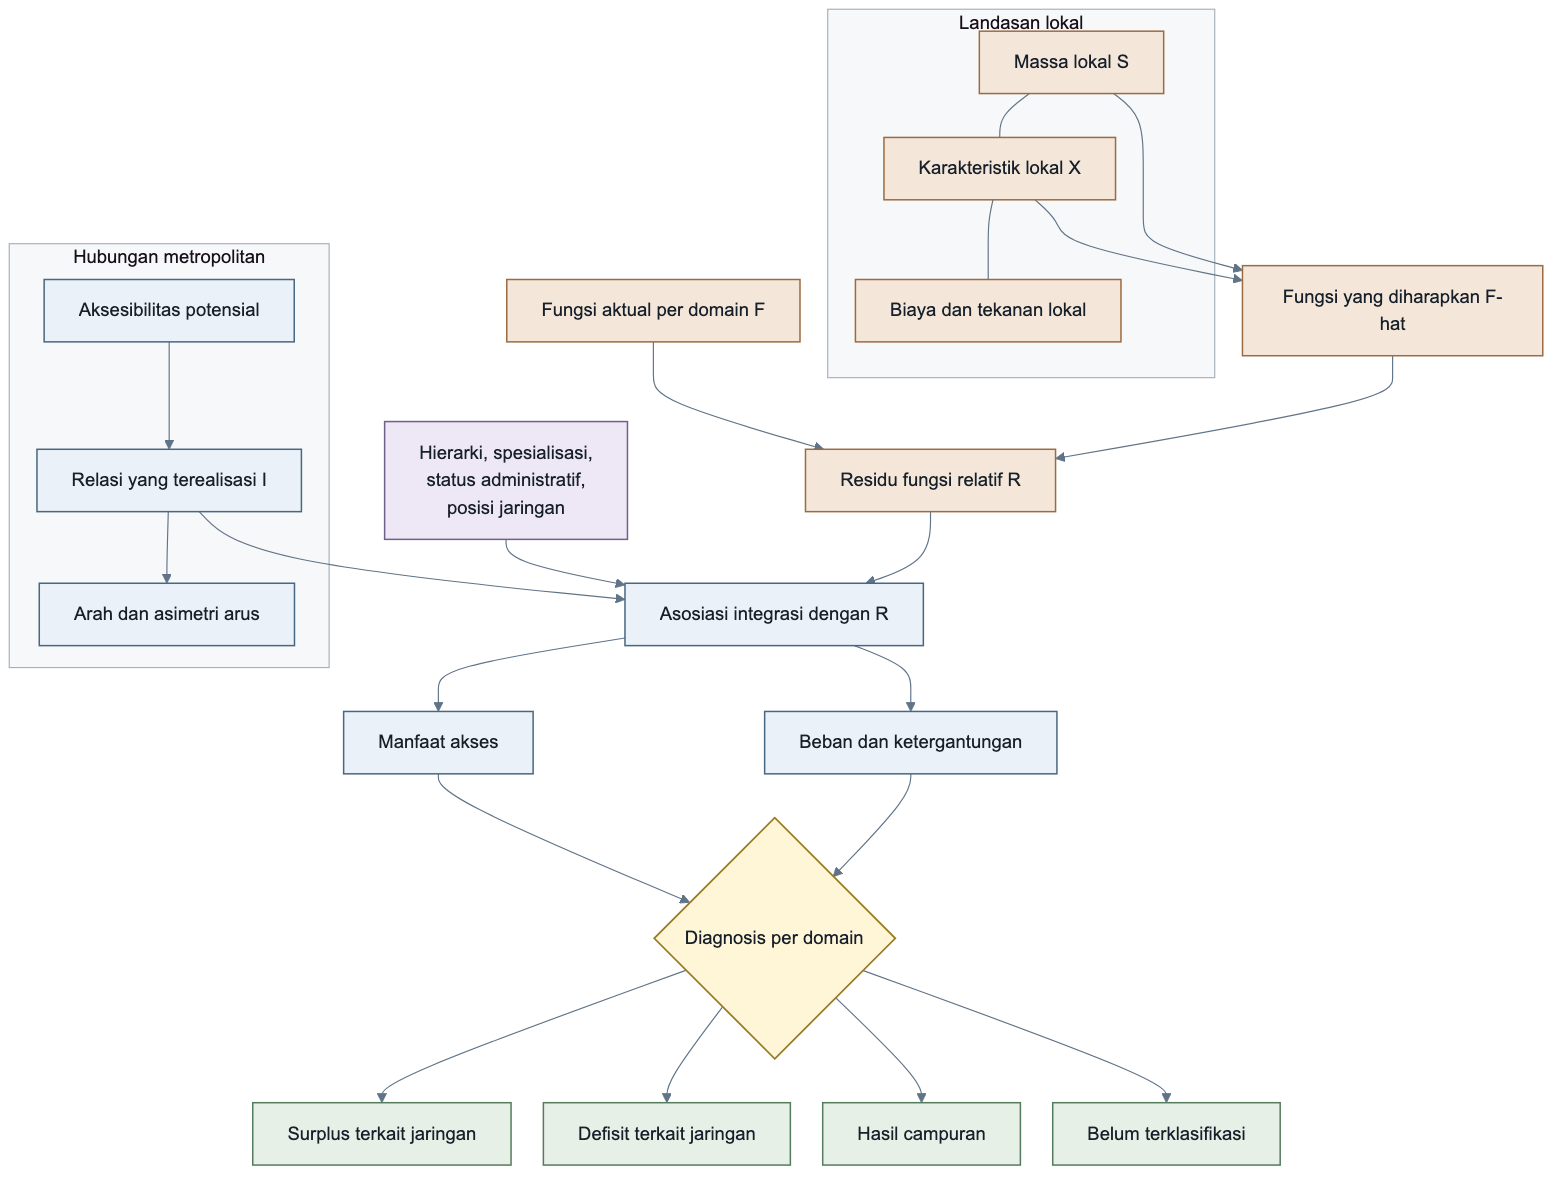
\includegraphics[width=0.88\textwidth]{figures/bab2_kerangka_konseptual.png}
  \caption{Kerangka konseptual hubungan massa lokal, relasi metropolitan, fungsi relatif, manfaat, beban, dan diagnosis per domain. Panah menunjukkan urutan pengukuran dan hubungan yang diuji, bukan hubungan kausal yang telah terbukti.}
  \label{fig:bab2-kerangka-konseptual}
\end{figure}

\subsection{Model pengukuran konseptual}

Untuk setiap pusat $i$ dan domain fungsi $k$, penelitian membedakan:

\begin{enumerate}
  \item Ukuran dan karakteristik lokal $(S_i,X_i)$;
  \item Integrasi relasional $(I_i)$ yang idealnya berasal dari arus atau interaksi;
  \item Fungsi aktual $(F_{ik})$;
  \item Fungsi yang diharapkan $(\widehat{F}_{ik})$;
  \item Residu fungsi relatif $(R_{ik})$;
  \item Manfaat akses $(A_{ik})$;
  \item Beban atau ketergantungan $(D_{ik})$; dan
  \item Ketahanan klasifikasi $(Q_i)$ berdasarkan variasi spesifikasi yang masih masuk akal.
\end{enumerate}

Hubungan konseptualnya dapat ditulis sebagai:

\[
R_{ik}=g_k(I_i,S_i,X_i,Z_i)+\varepsilon_{ik},
\]

\noindent dengan $Z_i$ sebagai moderator kontekstual. Persamaan ini bukan komitmen pada model kausal. Ia hanya menunjukkan objek yang perlu dipisahkan pada Bab 3: fungsi relatif sebagai keluaran, ukuran dan karakteristik lokal sebagai garis dasar, integrasi sebagai relasi, serta moderator dan ketidakpastian sebagai konteks.

\subsection{Tipologi diagnosis sementara}

\begin{table}[H]
\centering
\caption{Tipologi diagnosis berdasarkan relasi, fungsi relatif, dan beban}
\label{tab:tipologi}
\begin{adjustbox}{max width=\textwidth}
\begin{tabular}{p{0.18\textwidth}p{0.14\textwidth}p{0.18\textwidth}p{0.20\textwidth}p{0.24\textwidth}}
\toprule
\textbf{Integrasi} & \textbf{Residu} & \textbf{Beban} & \textbf{Kelas sementara} & \textbf{Interpretasi aman}\\
\midrule
Tinggi & Positif & Rendah hingga sedang & \textit{Borrowed size} atau integrasi produktif & Pola konsisten dengan akses jaringan yang memperbesar fungsi relatif.\\
Tinggi & Positif & Tinggi & Campuran atau \textit{contested} & Surplus hadir, tetapi manfaat disertai ketergantungan atau beban.\\
Tinggi & Negatif & Tinggi dan diukur terpisah dari residu & \textit{Agglomeration shadow} atau ketergantungan asimetris & Integrasi disertai defisit fungsi serta bukti beban atau ketergantungan yang independen.\\
Tinggi & Negatif & Rendah atau belum terbukti & Terintegrasi tetapi tertinggal & Belum cukup bukti untuk label \textit{shadow}.\\
Rendah & Positif & Bervariasi & Relatif independen atau matang lokal & Surplus tidak terutama dibaca sebagai hasil hubungan dengan Jakarta.\\
Rendah & Negatif & Bervariasi & Periferi lemah & Basis lokal dan hubungan metropolitan sama-sama terbatas.\\
\bottomrule
\end{tabular}
\end{adjustbox}
\end{table}

Kelas akhir dibentuk setelah indikator, arah hubungan, kualitas data, dan sensitivitas diperiksa. Residu fungsi tidak dihitung kembali sebagai indikator beban. Indeks komposit hanya digunakan apabila penggabungan tersebut tidak menyembunyikan perbedaan domain. Jika hasil tidak stabil, unit dilaporkan sebagai belum terselesaikan, bukan sebagai kondisi campuran substantif.

\subsection{Proposisi empiris}

Proposisi berikut menjadi panduan pengujian, bukan hipotesis kausal yang harus dipaksakan:

\begin{enumerate}
  \item Setelah ukuran dan karakteristik lokal diperhitungkan, integrasi fungsional yang lebih kuat dapat berasosiasi dengan surplus pada sebagian fungsi, tetapi tidak harus pada semua fungsi.
  \item Pada pusat tertentu, integrasi yang kuat dapat berasosiasi dengan defisit fungsi relatif dan beban ketergantungan yang lebih tinggi.
  \item Arah dan besar hubungan dapat berbeda antara pekerjaan, layanan, amenitas, fungsi keputusan, dan kinerja.
  \item Basis lokal, sentralitas, dan kapasitas penyerapan yang lebih kuat dapat membantu pusat mengubah akses jaringan menjadi pematangan fungsi.
  \item Polisentrisitas morfologis tidak dengan sendirinya menjelaskan integrasi fungsional, surplus fungsi, atau rendahnya ketergantungan.
  \item Sebagian unit dapat berpindah kelas ketika proksi, bobot, ambang, atau wilayah tangkapan diubah; unit yang stabil lebih layak menjadi dasar interpretasi.
\end{enumerate}

\subsection{Gerbang penggunaan label}

Label \textit{borrowed size} atau \textit{agglomeration shadow} digunakan hanya jika empat syarat terpenuhi:

\begin{enumerate}
  \item Terdapat bukti relasional atau estimasi yang diperiksa terhadap bukti independen;
  \item Fungsi aktual dibandingkan dengan ekspektasi ukuran pada unit pembanding yang memadai;
  \item Unit, periode, wilayah tangkapan, populasi sasaran, dan konstruk cukup kompatibel; dan
  \item Hasil tidak bergantung pada satu proksi lemah atau satu keputusan teknis.
\end{enumerate}

Tolok ukur utama menggunakan pusat sekunder Jabodetabek yang sebanding
dan menghasilkan posisi relatif internal. Khusus label
\textit{agglomeration shadow}, residu negatif harus disertai indikator
beban atau ketergantungan yang diukur terpisah dari residu. Tanpa bukti
tersebut, hasil disebut terintegrasi tetapi tertinggal.

Jika salah satu syarat gagal, istilah yang dipakai adalah aksesibilitas potensial, surplus atau defisit fungsi relatif, ketergantungan komuter, atau pola yang belum terklasifikasi. Aturan ini menjaga agar bahasa teori tidak melampaui status bukti.

\subsection{Posisi penelitian}

Penelitian ini membaca Jabodetabek sebagai sistem metropolitan dengan inti dominan dan sejumlah kandidat pusat sekunder. Relasi antarpusat dapat saling melengkapi, bersaing, atau bergantung. Sumber terbuka dan proksi menjadi dasar pengukuran karena dapat menyediakan lokasi, atribut, jaringan, dan seri waktu yang lebih mudah diulang daripada sumber resmi yang tersedia secara terputus. Keunggulan proksi tetap diuji melalui kesesuaian konstruk, cakupan, keterulangan, biaya, validasi terbuka, dan sensitivitas.

Bab 3 menerjemahkan kerangka ini ke dalam operasionalisasi. Observasi dipisahkan dari agregat, proksi, estimasi, dan simulasi. Periode hanya dibandingkan ketika serinya sebanding. Keluaran yang tidak memenuhi gerbang bukti dilaporkan sebagai diagnosis terbatas. Kerangka teoretis ini tidak menjanjikan panel lengkap atau hubungan kausal yang belum didukung data.

\clearpage

\chapter{Metode Penelitian}
\section{Pendekatan penelitian}\label{pendekatan-penelitian}

\subsection{Pilihan pendekatan}\label{pilihan-pendekatan}

Penelitian ini menggunakan pendekatan kuantitatif deduktif dengan
analisis spasial-relasional. Konstruk integrasi metropolitan,
fungsi relatif, manfaat, beban, serta gerbang penggunaan label
\emph{borrowed size} dan \emph{agglomeration shadow} diturunkan dari
kerangka konseptual Bab 2 sebelum klasifikasi dilakukan. Pendekatan ini
dipilih karena pertanyaan penelitian menuntut pengukuran hubungan antara
pusat sekunder dan Jakarta, perbandingan fungsi aktual dengan fungsi
yang diharapkan dari ukuran lokal, serta pengujian stabilitas hasil pada
variasi asumsi.

Pendekatan ini tidak berarti semua konstruk harus direduksi menjadi satu
angka. Integrasi, fungsi relatif, manfaat, ketergantungan, dan beban
dipertahankan sebagai dimensi yang dapat dibaca bersama. Statistik
deskriptif, pemetaan, analisis jaringan, tolok ukur, residu, dan uji
sensitivitas digunakan sesuai jenis bukti yang tersedia.

Audit dokumen dan audit asal-usul data merupakan prosedur penjaminan
mutu. Prosedur ini digunakan untuk memeriksa definisi, tahun, unit,
cakupan, cara pembentukan, nilai hilang, dan batas penggunaan data.
Pemeriksaan dokumen tersebut tidak menjadikan penelitian ini penelitian
campuran karena dokumen tidak dianalisis sebagai data untuk menjawab
pertanyaan substantif. Angka dalam laporan publik dapat diekstrak sebagai
data sekunder apabila tabel atau pernyataan sumber, unit, dan periodenya
dapat ditelusuri. Kekosongan angka tidak diisi dengan dugaan yang
disamarkan sebagai pengamatan.

\subsection{Alasan kesesuaian dengan pertanyaan
penelitian}\label{alasan-kesesuaian-dengan-pertanyaan-penelitian}

Kesesuaian pendekatan dengan pertanyaan penelitian diringkas sebagai
berikut.

{\def\LTcaptype{none} % do not increment counter
\begin{longtable}[]{@{}
  >{\raggedright\arraybackslash}p{(\linewidth - 4\tabcolsep) * \real{0.3333}}
  >{\raggedright\arraybackslash}p{(\linewidth - 4\tabcolsep) * \real{0.3333}}
  >{\raggedright\arraybackslash}p{(\linewidth - 4\tabcolsep) * \real{0.3333}}@{}}
\toprule\noalign{}
\begin{minipage}[b]{\linewidth}\raggedright
Kode
\end{minipage} & \begin{minipage}[b]{\linewidth}\raggedright
Fokus pertanyaan
\end{minipage} & \begin{minipage}[b]{\linewidth}\raggedright
Alasan menggunakan pendekatan kuantitatif-spasial
\end{minipage} \\
\midrule\noalign{}
\endhead
\bottomrule\noalign{}
\endlastfoot
Q1 & Arah, intensitas, dan asimetri hubungan metropolitan & Pengamatan
dan estimasi relasi dari sumber terbuka dibandingkan pada unit yang
sah. \\
Q2 & Fungsi relatif, manfaat, beban, dan perubahan pada seri sebanding &
Pengukuran atau estimasi fungsi dibandingkan dengan tolok ukur, sementara
manfaat dan beban dilaporkan pada penerima serta penanggungnya. \\
Q3 & Hubungan integrasi dan fungsi relatif serta konfigurasi hasil &
Asosiasi, heterogenitas antarpusat, sirkularitas, kondisi lokal, dan
penjelasan alternatif diperiksa sebelum diagnosis. \\
\end{longtable}
}

Sensitivitas menjadi pemeriksaan lintas ketiga pertanyaan, bukan
pertanyaan substantif tersendiri.

Pendekatan ini tidak cukup untuk menyatakan dampak kausal pembangunan
jalan, perluasan wilayah, atau kebijakan tertentu tanpa strategi
identifikasi tambahan. Karena itu, istilah yang dipakai dalam Bab 3
adalah \emph{asosiasi}, \emph{pola}, \emph{surplus atau defisit
relatif}, \emph{ketergantungan yang konsisten dengan data}, dan
\emph{ketahanan klasifikasi}, bukan ``dampak kausal'' kecuali desain
kelak benar-benar diperkuat.

\subsection{Fondasi pengukuran}\label{fondasi-pengukuran}

Penelitian ini sepenuhnya bertumpu pada proksi dan sumber terbuka, tanpa
ketergantungan pada permohonan data tertutup. Data pemerintah yang
terbuka tetap dapat digunakan. Pemilihan sumber mengikuti kesesuaian
konstruk, cakupan spasial dan temporal, keterulangan pengolahan, serta
biaya pemerolehan; status resmi tidak menjadi ukuran mutu dengan
sendirinya. Sumber alternatif dapat lebih sesuai daripada data resmi
agregat yang tersedia, tetapi keunggulan tersebut diuji per konstruk dan
tidak diasumsikan berlaku universal.

\section{Desain penelitian}\label{desain-penelitian}

\subsection{Bentuk desain}\label{bentuk-desain}

Penelitian dirancang sebagai studi kasus tunggal kuantitatif-spasial
dengan pengamatan multitemporal sesuai bukti, diagnosis relasional, dan
analisis sensitivitas. Kasus tunggal dipilih agar pusat-pusat sekunder
dapat dibandingkan di dalam satu sistem metropolitan tanpa memperlakukan
perbedaan antarmetropolitan sebagai variasi yang setara. Populasi
pembanding utama adalah pusat-pusat sekunder di dalam Jabodetabek yang
memiliki konstruk, unit, dan periode sebanding. DKI Jakarta dikeluarkan
dari pembentukan ekspektasi karena kedudukannya sebagai inti. Sabuk
pembanding di luar kawasan studi hanya digunakan sebagai pemeriksaan
sensitivitas apabila definisi, unit, dan periodenya kompatibel.

Desain ini bekerja melalui tiga lapisan:

\begin{enumerate}
\def\labelenumi{\arabic{enumi}.}
\tightlist
\item
  Lapisan pengukuran membedakan observasi langsung atau agregat, proksi,
  serta hasil estimasi yang dibedakan secara eksplisit pada unit dan
  periode yang tercantum dalam manifest.
\item
  Lapisan diagnosis mengukur integrasi, fungsi relatif,
  manfaat, beban, dan tipologi dari satu konfigurasi bukti yang
  dibekukan.
\item
  Lapisan ketahanan dan eksplorasi menguji perubahan konfigurasi
  bukti, spesifikasi model, atau nilai skenario yang dibatasi dan selalu
  dilaporkan terhadap garis dasar tanpa menimpa data observasi.
\end{enumerate}

\subsection{Urutan kerja
penelitian}\label{urutan-kerja-penelitian}

Penelitian dilaksanakan melalui delapan tahap yang saling terkait.

\begin{enumerate}
\def\labelenumi{\arabic{enumi}.}
\tightlist
\item
  Menginventarisasi sumber dan mencatat asal-usul setiap data.
\item
  Mengaudit konstruk, tahun, unit, cakupan, lisensi, nilai hilang, dan
  batas penggunaan.
\item
  Mengharmonisasi geometri dan tabel, kemudian membekukan konfigurasi
  bukti garis dasar.
\item
  Membentuk kandidat pusat, wilayah tangkapan, relasi terarah, dan
  residu fungsi per domain.
\item
  Menganalisis asosiasi, manfaat, beban, dan ketergantungan tanpa
  meleburkan dimensi yang berbeda.
\item
  Menerapkan gerbang bukti sebelum memberi label diagnosis.
\item
  Menguji sensitivitas indikator, bobot, ambang, unit, dan konfigurasi
  bukti.
\item
  Menyusun tabel, peta, manifest, dan batas klaim yang dapat diperiksa
  ulang; Web GIS interaktif hanya disiapkan jika keluaran inti telah
  selesai dan waktu penelitian memungkinkan.
\end{enumerate}

\begin{figure}[H]
  \centering
  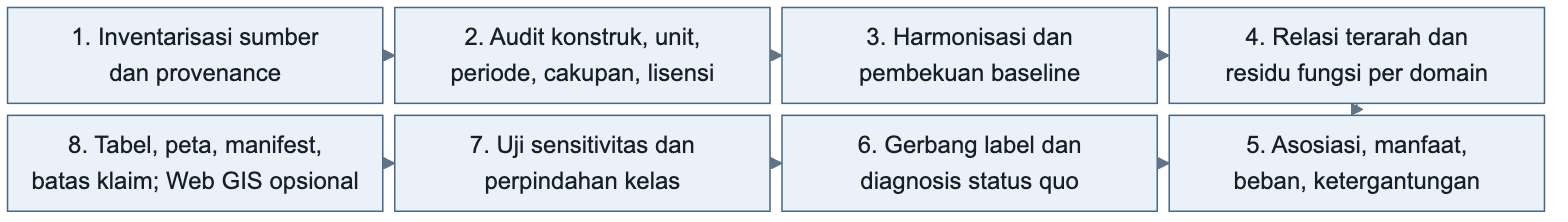
\includegraphics[width=\textwidth]{figures/bab3_alur_analisis.png}
  \caption{Alur analisis dari inventarisasi sumber hingga penyusunan keluaran dan batas klaim. Setiap tahap dapat menurunkan tingkat klaim jika mutu atau keterbandingan bukti tidak memadai.}
  \label{fig:bab3-alur-analisis}
\end{figure}

\subsection{Rancangan analisis minimum}\label{rancangan-analisis-minimum}

Rancangan minimum dibatasi pada satu periode yang kompatibel, satu bukti
relasi komuter terarah, satu domain fungsi yang dibentuk secara
independen, tolok ukur internal Jabodetabek, serta pembacaan hubungan
antara relasi dan residu fungsi. Domain pekerjaan menjadi pilihan utama
jika pasangan arus komuter diamati tanpa dibentuk dari estimasi pekerjaan
yang sama. Layanan berorde tinggi dapat menjadi domain kedua apabila
atributnya lolos audit dan tidak digunakan untuk membentuk relasi.

Jika jumlah pusat efektif tidak memadai untuk regresi, keluaran minimum
berupa profil terarah dan perbandingan kelompok. Analisis multitemporal,
domain kedua, CCTV, SUMO, dan Web GIS interaktif dilaksanakan setelah
rantai utama tersebut berjalan dan tidak menjadi syarat untuk menjawab
pertanyaan inti. Kategori diagnosis hanya dibentuk jika keempat gerbang
bukti terpenuhi; hasil lain tetap sah sebagai profil relasi serta surplus
atau defisit fungsi relatif.

\subsection{Kelebihan dan keterbatasan
desain}\label{kelebihan-dan-keterbatasan-desain}

Desain memungkinkan pengukuran spasial terperinci dan pengamatan
beberapa periode dari sumber yang dapat diperiksa tanpa menunggu akses
kelembagaan. Keterbatasan data administratif maupun nonpemerintah
dinilai secara simetris. Ketersediaan koordinat, panjang seri, dan
banyaknya sumber merupakan keunggulan hanya sejauh membantu mengukur
konstruk yang dituju.

Galat klasifikasi usaha, duplikasi, cakupan yang berbeda antardaerah,
perubahan pencatatan, dan asumsi model dapat memengaruhi hasil.
Pemeriksaan independen, harmonisasi, serta propagasi ketidakpastian
digunakan untuk mengukur pengaruhnya. Data multitemporal tidak dengan
sendirinya mengidentifikasi sebab-akibat.

\subsection{Perbedaan diagnosis dan
skenario}\label{perbedaan-diagnosis-dan-skenario}

Nilai \emph{status quo} dibekukan sebagai garis dasar. Perubahan
penggeser atau parameter tidak boleh menimpa nilai observasi, mengubah
batas administratif, atau disajikan sebagai prediksi. Setiap skenario
menyimpan konfigurasi indikator, bobot, ambang, nilai yang diubah, dan
alasan substantif perubahan.

Perubahan karena sumber data diperoleh, hilang, atau turun mutu dicatat
sebagai skenario bukti. Perubahan bobot, ambang, atau
spesifikasi dalam konfigurasi bukti yang sama dicatat sebagai
skenario parameter. Perubahan nilai indikator untuk pertanyaan
\emph{what-if} merupakan eksplorasi kondisional tambahan. Ketiganya
tidak boleh ditampilkan sebagai jenis perubahan yang sama.

\section{Ruang lingkup penelitian}\label{ruang-lingkup-penelitian}

\subsection{Ruang lingkup spasial}\label{ruang-lingkup-spasial}

Kasus utama adalah Jabodetabek sebagai kawasan utama penelitian. Tolok
ukur utama dibentuk dari pusat sekunder yang sebanding di dalam kawasan
ini. Sabuk Wilayah Statistik Metropolitan di luar cakupan hanya menjadi
pemeriksaan sensitivitas apabila datanya kompatibel. Kasus ini dipilih karena memungkinkan
hubungan antara satu inti dan kandidat pusat sekunder lintas batas
administratif diperiksa di dalam sistem metropolitan yang sama. DKI
Jakarta diperlakukan sebagai satu inti untuk hubungan eksternal, dengan
batas administratif tetap. Data rinci di dalam DKI tetap dapat digunakan
untuk pemeriksaan internal, tetapi tidak mengubah keputusan bahwa DKI
diperlakukan sebagai satu inti dalam klasifikasi eksternal.

Wilayah di luar DKI tidak disebut sebagai ``wilayah Jakarta'' hanya
karena masuk dalam gradien analisis. Istilah yang digunakan adalah
jejak fungsional Jakarta, zona analitis keterkaitan metropolitan, atau
gradien integrasi-ketergantungan metropolitan. Istilah tersebut bukan zonasi legal RTRW dan tidak
mengubah kewenangan pemerintah daerah.

Seluruh wilayah administratif di sekitar Jakarta tidak diasumsikan
otomatis menjadi unit analisis yang tepat. Delineasi akhir harus
menjelaskan sumber, tahun, definisi, dan alasan memasukkan atau
mengeluarkan setiap unit.

\subsection{Ruang lingkup temporal}\label{ruang-lingkup-temporal}

Desain penelitian bersifat multitemporal sesuai bukti: perubahan
dianalisis pada indikator dengan seri yang sebanding, sedangkan
indikator lain dianalisis pada periode yang tersedia. Tahun dasar dan
rentang analisis ditetapkan per modul setelah audit; panel lengkap dan
satu tahun jangkar untuk semua sumber tidak diasumsikan.

Setiap modul menyimpan tahun observasi, tanggal ekstraksi, waktu
publikasi, dan periode berlakunya atribut. Analisis perubahan
mensyaratkan sedikitnya dua pengamatan yang sebanding; dua titik tidak
disebut tren tahunan. Riwayat suntingan OSM dan tanggal kemunculan dalam
direktori bukan otomatis tanggal berdiri atau tutup usaha. Data mutakhir
tidak diproyeksikan ke masa lalu tanpa model dan bukti. Seri tidak
sebanding dianalisis terpisah; interpolasi, jika digunakan, diberi label
estimasi dan tidak menambah jumlah observasi independen.

\subsection{Ruang lingkup
substantif}\label{ruang-lingkup-substantif}

Penelitian mencakup:

\begin{itemize}
\tightlist
\item
  Integrasi atau eksposur metropolitan;
\item
  Fungsi lokal dan fungsi relatif pada satu atau paling banyak dua
  domain inti;
\item
  Manfaat akses yang dapat diamati atau diproksikan secara sah;
\item
  Beban komuter dan ketergantungan yang diukur terpisah dari residu
  fungsi;
\item
  Tipologi \emph{borrowed size}, campuran,
  \emph{agglomeration shadow}, terintegrasi tetapi tertinggal, relatif
  independen, periferi lemah, dan tidak terselesaikan;
\item
  Sensitivitas indikator, bobot, ambang, unit, dan status mutu bukti;
  serta
\item
  Penyajian hasil dalam atlas, tabel, dan peta; Web GIS interaktif dapat
  ditambahkan sebagai media komunikasi.
\end{itemize}

Penelitian tidak mencakup penetapan radius geometris Jakarta,
rekomendasi perubahan batas administrasi, pembuktian kausal seluruh
kebijakan metropolitan, atau klaim produktivitas penuh jika fungsi
ekonomi pada unit yang sesuai tidak tersedia.

Kematangan dalam penelitian ini berarti kematangan fungsi lokal pada
domain yang benar-benar diukur. Konstruk tersebut tidak disamakan dengan
kesejahteraan penduduk, keterjangkauan layanan, mutu pelayanan secara
menyeluruh, ketahanan ekonomi, atau keberhasilan pembangunan. Akses,
manfaat, dan beban dilaporkan terpisah dan tidak digunakan untuk
memperluas arti residu fungsi.

\section{Unit amatan dan unit
analisis}\label{unit-amatan-dan-unit-analisis}

\subsection{Unit amatan}\label{unit-amatan}

Unit amatan adalah satuan tempat setiap observasi dicatat pada sumber.
Satuan tersebut dapat berupa desa/kelurahan, kecamatan, kabupaten/kota,
zona asal-tujuan, titik fasilitas, atau sel raster. Kecamatan menjadi
sasaran unit amatan utama untuk modul yang memiliki bukti relasional dan
fungsi yang kompatibel karena cukup rinci untuk membedakan kandidat
pusat sekunder dan wilayah sekitarnya.

Kecamatan tidak dipaksakan ketika data kritis hanya tersedia pada
kabupaten/kota atau zona model. Dalam keadaan tersebut, perhitungan
dilakukan pada unit sumber atau sebagai analisis paralel multiresolusi.
Alokasi nilai kabupaten/kota ke kecamatan, kisi, atau titik hanya
dilakukan dengan model eksplisit menggunakan informasi lokal, pemeriksaan
independen, dan ketidakpastian; hasil tetap merupakan estimasi, bukan
observasi rinci.

Kisi atau heksagon hanya digunakan untuk data yang berasal dari raster
atau titik, misalnya cahaya malam, morfologi terbangun, atau titik
minat. Kisi dapat menjadi unit perhitungan utama bagi modul yang
didukung titik atau raster. Resolusi keluaran mengikuti kemampuan
pengukuran; koordinat rinci tidak otomatis menjamin ketepatan nilai
atribut.

\subsection{Unit analisis
substantif}\label{unit-analisis-substantif}

Unit analisis substantif adalah kandidat pusat sekunder beserta wilayah
tangkapan fungsionalnya. Secara operasional, satu pusat dapat
direpresentasikan oleh satu kecamatan, beberapa unit yang bersebelahan,
atau zona sumber selama aturan pembentukannya dibekukan dan dapat
direproduksi. Kabupaten/kota tetap menjadi lapisan agregasi kebijakan,
layanan, APBD, dan tanggung jawab pemerintahan, tetapi tidak otomatis
menjadi pusat sekunder.

Daftar kandidat awal dibentuk dari konsentrasi aktivitas dan fungsi
dalam sumber terbuka, serta dibandingkan dengan pusat yang dikenali
dalam dokumen perencanaan. Penetapannya menggunakan bukti kepadatan
aktivitas, fungsi layanan, pekerjaan, kawasan industri, posisi jaringan,
atau arus yang tersedia. Variabel untuk delineasi dipisahkan dari
variabel hasil sejauh data memungkinkan. Jika indikator yang sama harus
digunakan pada kedua tahap, ketahanan klasifikasi diuji kembali dengan
mengeluarkan indikator tersebut agar penetapan pusat tidak menjadi
pembuktian sirkular.

\subsection{Aturan keterbandingan
unit}\label{aturan-keterbandingan-unit}

Setiap indikator dicatat dengan unit asli, unit perhitungan, unit
pelaporan, dan operasi transformasinya. Satu klasifikasi hanya dihitung
jika bukti relasional dan bukti fungsi dapat dipadankan pada unit,
wilayah tangkapan, dan periode yang sebanding atau dapat diagregasikan
secara sah. Harmonisasi mengikuti aturan:

\begin{enumerate}
\def\labelenumi{\arabic{enumi}.}
\tightlist
\item
  Gunakan unit asli untuk perhitungan awal;
\item
  Gunakan tabel korespondensi resmi jika tersedia;
\item
  Agregasikan unit rinci ke unit lebih kasar bila operasi tersebut sah;
\item
  Jalankan analisis paralel bila unit tidak dapat disetarakan;
\item
  Keluarkan modul jika keterbandingan tidak dapat dipertanggungjawabkan;
  dan
\item
  Jangan membandingkan skor lintas konfigurasi bukti sebagai perubahan
  kondisi tanpa menyatakan perbedaan sumber dan unitnya.
\end{enumerate}

\subsection{Populasi, cakupan, dan validasi
manual}\label{populasi-cakupan-dan-validasi-manual}

Populasi analisis adalah seluruh kandidat pusat dan wilayah tangkapan
yang masuk dalam delineasi akhir serta mempunyai bukti yang memenuhi
aturan modul. Jika sumber merupakan sensus atau inventaris seluruh unit,
penelitian tidak mengambil sampel statistik tambahan. Pemeriksaan manual
dilakukan secara purposif pada tiga sampai lima pusat sekunder prioritas
untuk memeriksa lokasi kampus dan rumah sakit; usaha dan titik minat
lain diperiksa pada sampel terarah yang mencakup variasi sektor,
koridor, dan tingkat ketercakupan. Audit silang memeriksa asal-usul
sumber agar dua salinan data yang sama tidak dianggap dua bukti
independen. Kriteria pemilihan pusat validasi dicatat sebelum
pemeriksaan. Validasi terbatas tersebut bukan sampel inferensial dan
tidak digeneralisasikan sebagai sensus seluruh kawasan.

Untuk tolok ukur fungsi, populasi pembanding garis dasar menggunakan
seluruh pusat sekunder yang lolos aturan keterbandingan pada domain yang
sama. Nilai suatu pusat diperkirakan dari pusat pembanding lain dengan
prosedur \emph{leave-one-out} agar pengamatan yang sedang dinilai tidak
menentukan ekspektasinya sendiri. Jika jumlah pusat tidak mendukung model
fungsi-ukuran, pembanding dibentuk dari kelompok ukuran atau tetangga
ukuran terdekat yang transparan. Kedua prosedur tetap menghasilkan
posisi relatif di dalam Jabodetabek.

\section{Metode pengumpulan data}\label{metode-pengumpulan-data}

\subsection{Prinsip pengumpulan
data}\label{prinsip-pengumpulan-data}

Penelitian ini sepenuhnya bertumpu pada proksi dan sumber terbuka, tanpa
ketergantungan pada permohonan data tertutup. Data pemerintah yang
terbuka tetap dapat digunakan. Pemilihan sumber mengikuti kesesuaian
konstruk, cakupan spasial dan temporal, keterulangan pengolahan, serta
biaya pemerolehan; status resmi tidak menjadi ukuran mutu dengan
sendirinya.

Akuisisi mengikuti sumber yang benar-benar dapat digunakan: unduhan,
layanan data, direktori publik, laporan operator, publikasi statistik,
serta ekstraksi dokumen dengan locator tabel atau halaman. Metode
pengambilan OSM dan Google Maps ditetapkan setelah audit kemampuan
akses; penelitian tidak menganggap satu endpoint pencarian sebagai
satu-satunya cara akuisisi atau hasil pencarian sebagai sensus lengkap.
Terlihat publik tidak otomatis berarti tersedia sebagai unduhan terbuka
atau dapat dibagikan ulang; kemampuan akuisisi dan reproduksi dicatat
per sumber.

\subsection{Kelompok sumber dan konstruksi
data}\label{kelompok-sumber-dan-konstruksi-data}

Tabel berikut adalah rancangan sumber yang perlu diperiksa. Penyebutan
sumber tidak menyatakan bahwa seri, atribut, atau cakupan seluruh
Jabodetabek telah tersedia.

{\def\LTcaptype{none} % do not increment counter
\begin{longtable}[]{@{}
  >{\raggedright\arraybackslash}p{(\linewidth - 4\tabcolsep) * \real{0.3333}}
  >{\raggedright\arraybackslash}p{(\linewidth - 4\tabcolsep) * \real{0.3333}}
  >{\raggedright\arraybackslash}p{(\linewidth - 4\tabcolsep) * \real{0.3333}}@{}}
\toprule\noalign{}
\begin{minipage}[b]{\linewidth}\raggedright
Modul
\end{minipage} & \begin{minipage}[b]{\linewidth}\raggedright
Kandidat sumber terbuka
\end{minipage} & \begin{minipage}[b]{\linewidth}\raggedright
Konstruksi pengukuran dan pemeriksaan
\end{minipage} \\
\midrule\noalign{}
\endhead
\bottomrule\noalign{}
\endlastfoot
Batas dan massa lokal & BIG, publikasi BPS, sumber pemda, raster
penduduk & Geometri, penduduk, dan karakteristik lokal; samakan
definisi, tahun, serta batas. \\
Usaha dan pekerjaan & OSM, Overture, Google Maps yang dapat digunakan,
direktori usaha, bangunan, publikasi sektoral & Deduplicasi dan padankan
lokasi serta kategori; estimasikan pekerjaan dari koefisien beralasan,
skala bangunan, dan informasi usaha. \\
Fungsi layanan & Direktori fasilitas, PDDikti, SIRS, sumber kelas atau
akreditasi publik & Padankan lokasi fisik, kelas, spesialisasi,
kapasitas, dan akreditasi beserta masa berlakunya; jumlah fasilitas dan
mutu tidak disamakan. \\
Jaringan dan layanan angkutan & OSM, GTFS yang tersedia, laporan
TransJakarta, MRT, LRT, KRL, dan publikasi transportasi & Pisahkan rute,
frekuensi, armada, kapasitas, penumpang, serta waktu; cakupan operator
tidak dianggap mewakili semua moda. \\
Relasi terarah & Tabulasi komuter publik, WSM, laporan BPTJ/JUTPI yang
terbuka, informasi operator & Gunakan observasi pada resolusi sumber
atau kendala bagi estimasi OD; marginal dan kapasitas bukan pasangan
arus aktual. \\
Ekonomi dan morfologi & PDRB publik, direktori kawasan industri, GHSL,
WorldPop, VIIRS, citra terbuka & Konteks sektor, keterbangunan, dan
aktivitas; produktivitas hanya diestimasi apabila pembilang dan penyebut
kompatibel. \\
Pemeriksaan tambahan & Sumber terbuka independen, dokumentasi lokasi,
dan rekaman CCTV yang tersedia & Periksa cakupan waktu dan lokasi;
deteksi serta pelacakan objek dan SUMO merupakan penguatan yang harus
melewati audit dan validasi, bukan syarat terlaksananya penelitian. \\
\end{longtable}
}

Apabila definisi atau ambang suatu publikasi bertentangan, simpan versi
dan locator yang relevan, gunakan hanya variabel yang dapat ditafsirkan,
dan uji alternatif yang masuk akal. Penelitian tidak menunggu jawaban
instansi untuk menggunakan modul lain yang sudah dapat
dipertanggungjawabkan.

\subsection{Instrumen pengumpulan dan dokumentasi
data}\label{instrumen-pengumpulan-dan-dokumentasi-data}

Karena penelitian menggunakan data sekunder, instrumen pengumpulan bukan
kuesioner atau panduan wawancara. Instrumen kerja terdiri atas:

\begin{enumerate}
\def\labelenumi{\arabic{enumi}.}
\tightlist
\item
  Log akses untuk mencatat alamat sumber, tanggal akses, dan syarat
  penggunaan;
\item
  Formulir audit berkas dan registri asal-usul data;
\item
  Kamus data yang memuat definisi variabel, unit, tahun, nilai hilang,
  dan polaritas;
\item
  Tabel korespondensi kode serta geometri antarversi;
\item
  Manifest konfigurasi bukti dan parameter; serta
\item
  Lembar pemeriksaan manual untuk kampus dan rumah sakit, serta untuk
  sampel hasil penghitungan objek apabila modul CCTV dijalankan.
\end{enumerate}

Skrip akuisisi, pembersihan, transformasi, dan analisis diperlakukan
sebagai bagian dari instrumen yang dapat direproduksi. Nama perangkat
lunak, versi, parameter, dan tanggal pengolahan dicatat setelah
perangkat benar-benar digunakan; Bab 3 tidak mengunci perangkat yang
belum dipakai.

\subsection{Audit dan status mutu
bukti}\label{audit-dan-status-mutu-bukti}

Setiap berkas dicatat dalam registri asal-usul data sekurang-kurangnya
menurut sumber, nama/versi berkas, tanggal akses, tahun observasi, unit,
cakupan, definisi, metode pembentukan, nilai hilang, reliabilitas,
lisensi, dan pembatasan publikasi.

{\def\LTcaptype{none} % do not increment counter
\begin{longtable}[]{@{}
  >{\raggedright\arraybackslash}p{(\linewidth - 4\tabcolsep) * \real{0.3333}}
  >{\raggedright\arraybackslash}p{(\linewidth - 4\tabcolsep) * \real{0.3333}}
  >{\raggedright\arraybackslash}p{(\linewidth - 4\tabcolsep) * \real{0.3333}}@{}}
\toprule\noalign{}
\begin{minipage}[b]{\linewidth}\raggedright
Status
\end{minipage} & \begin{minipage}[b]{\linewidth}\raggedright
Nama
\end{minipage} & \begin{minipage}[b]{\linewidth}\raggedright
Aturan penggunaan
\end{minipage} \\
\midrule\noalign{}
\endhead
\bottomrule\noalign{}
\endlastfoot
D & Langsung & Konstruk teramati pada unit dan periode sasaran dengan
mutu memadai. \\
A & Agregat & Konstruk teramati, tetapi unit, waktu, kategori, atau
cakupan lebih kasar. \\
S & Sintetis & Nilai diestimasi dari data lain; asumsi, kalibrasi, dan
ketidakpastian wajib ditampilkan. \\
P & Proksi & Mengukur gejala terkait, bukan konstruk yang hendak diklaim
secara langsung. \\
\(\varnothing\) & Dikeluarkan & Tidak tersedia, tidak sebanding, tidak
reliabel, atau tidak dapat dipertanggungjawabkan. \\
\end{longtable}
}

Status tersebut menjelaskan cara pengukuran, bukan urutan mutu sumber.
Data resmi maupun nonpemerintah dapat mengandung galat. Pengamatan
langsung pada unit publikasi tidak otomatis merupakan pengamatan
langsung pada unit penelitian. Misalnya, survei kabupaten/kota dapat
berstatus A untuk penelitian berkecamatan; jaringan dapat berstatus P
untuk integrasi aktual; dan tabel bangkitan-tarikan dapat berstatus S
atau A jika tidak memuat pasangan arus teramati.

\subsection{Harmonisasi spasial dan
temporal}\label{harmonisasi-spasial-dan-temporal}

Harmonisasi dilakukan setelah audit, bukan sebelum audit. Tahun dasar
dan rentang perbandingan ditetapkan per modul setelah audit
kesebandingan. Variabel dari 2023 atau 2025 tidak dinormalisasi ulang
untuk menyembunyikan perbedaan tahun. Setiap peta, tabel, dan skor
menyimpan tahun sumber dan status perbandingannya.

Untuk data spasial, geometri unit asli dipertahankan dalam arsip kerja.
Tabel korespondensi resmi digunakan bila tersedia. Agregasi dari desa ke
kecamatan dapat dilakukan bila definisi, kode, dan cakupan mendukung.
Disagregasi nilai kabupaten/kota ke kecamatan dilarang kecuali ada model
eksplisit, asumsi terlihat, validasi, dan pelabelan sintetis.

\subsection{Konstruksi proksi dan
estimasi}\label{konstruksi-proksi-dan-estimasi}

Pekerjaan dapat diestimasi dari jenis dan skala usaha, bangunan yang
dipadankan, serta koefisien tenaga kerja dengan sumber yang dapat
diperiksa. Dasar koefisien, variasi sektor, usaha informal, duplikasi
cabang, tingkat hunian, dan lokasi kerja dibedakan. Koefisien dari
wilayah atau periode lain diuji rentangnya; angka tidak dibuat sekadar
untuk melengkapi tabel. Jika koefisien belum memiliki dasar, keluaran
sementara tetap berupa fungsi atau skala usaha.

Relasi asal dan tujuan dapat diestimasi dengan model gravitasi atau
radiasi. Penyeimbangan IPF/Furness digunakan hanya jika marginal asal
dan tujuan kompatibel dan totalnya konsisten atau penyesuaiannya
beralasan. Ketidakpastian fungsi hambatan, massa tujuan, pilihan moda,
dan arus internal diperiksa. Data yang digunakan untuk kalibrasi tidak
dilaporkan sebagai validasi independen. Kecocokan marginal tidak
membuktikan keunikan matriks OD.

Laporan tahunan dan berita dapat menyediakan informasi armada,
perjalanan, kapasitas, atau penumpang; setiap angka harus memiliki
periode, unit, dan rujukan yang jelas. Kapasitas kendaraan memerlukan
asumsi frekuensi, operasi, serta keterisian untuk memperkirakan
penggunaan.

Rekaman CCTV yang telah tersedia dapat digunakan untuk mengestimasi arus
pada titik dan interval waktu tertentu. Model YOLO pralatih mendeteksi
kelas objek, sedangkan pelacak objek mempertahankan identitas antarbingkai
agar satu kendaraan tidak dihitung berulang. Penghitungan dilakukan pada
garis atau wilayah pengamatan yang dibekukan, kemudian diagregasi menurut
kamera, waktu, arah, dan kelas objek. Sepeda motor, mobil, bus, truk,
sepeda, atau pejalan kaki hanya digunakan jika kelas tersebut dapat
dibedakan secara memadai pada rekaman.

Kelayakan modul CCTV ditentukan melalui sampel berlabel manual yang
mewakili kamera, kepadatan, cuaca, pencahayaan, sudut pandang, dan tingkat
oklusi. Pemeriksaan mencakup ketepatan deteksi, kehilangan atau pertukaran
identitas, galat jumlah, serta sensitivitas terhadap ambang keyakinan dan
aturan pelacakan. Hasilnya disebut estimasi hitungan berbasis rekaman,
bukan observasi tanpa galat dan bukan matriks asal dan tujuan. SUMO dapat
menggunakan hitungan yang kompatibel untuk kalibrasi simulasi; simulasi
tetap tidak menciptakan arus aktual atau pasangan asal dan tujuan yang
belum diamati.

Validasi menggunakan sumber terbuka dengan jalur pencatatan berbeda,
pengamatan terarah, atau data yang disisihkan dari kalibrasi. Jika
pemeriksaan independen belum tersedia, keluaran relasional dilaporkan
sebagai estimasi eksploratif dengan rentang ketidakpastian; keterbatasan
ini tidak menghentikan modul fungsi atau aksesibilitas yang valid.

\subsection{Etika, lisensi, dan
keamanan}\label{etika-lisensi-dan-keamanan}

Data yang dapat diakses publik tetap diperiksa syarat pemakaian,
privasi, dan hak penyebarluasan turunannya. Pengolahan CCTV menyimpan
hitungan agregat dan metadata yang diperlukan, bukan wajah, pelat nomor,
atau identitas individu. Keluaran Web GIS mengikuti izin publikasi setiap sumber. Peta publik hanya memuat
data yang boleh dipublikasikan, agregasi yang sah, atau proksi yang
diberi label. Nilai penggeser tidak boleh mengungkap data mentah atau
memungkinkan rekonstruksi unit sensitif.

\section{Metode analisis data}\label{metode-analisis-data}

\subsection{Langkah 1: audit, dokumentasi, dan pembekuan garis
dasar}\label{langkah-1-audit-dokumentasi-dan-pembekuan-garis-dasar}

Analisis dimulai dengan tabel audit yang menghubungkan konstruk,
indikator, sumber, tahun, unit, polaritas, status bukti, aturan
transformasi, dan batas klaim. Garis dasar dibekukan setelah tahap audit
awal agar skenario tidak mengubah nilai observasi.

Pada tahap ini ditetapkan pula indikator yang dikeluarkan karena
duplikasi, cakupan yang tidak memadai, proporsi nilai hilang yang
mengganggu keterbandingan, ketidakcocokan unit, atau ketidakjelasan
definisi. Pengeluaran indikator dicatat sebagai keputusan metodologis,
bukan dihapus tanpa jejak.

\subsection{Langkah 2: delineasi pusat sekunder dan wilayah
tangkapan
fungsional}\label{langkah-2-delineasi-pusat-sekunder-dan-wilayah-tangkapan-fungsional}

Kandidat pusat sekunder berangkat dari daftar yang dikenali dalam sumber
resmi, kemudian diuji dengan bukti fungsi dan hubungan yang tersedia.
Bukti yang dapat digunakan meliputi kepadatan aktivitas, fasilitas,
pekerjaan, kawasan industri, posisi jaringan, arus perjalanan, atau
kombinasi yang ditetapkan sebelum pengukuran fungsi relatif dan
klasifikasi.

Setiap kandidat diberi alasan masuk, sumber, unit, periode, dan tingkat
ketidakpastian. Aturan pembentukan wilayah tangkapan fungsional
dibekukan untuk setiap konfigurasi bukti sebelum hasil fungsi relatif
dihitung. Wilayah tangkapan dapat berbeda antarkonfigurasi bukti, tetapi
perubahan tersebut harus diberi versi dan tidak boleh ditampilkan
sebagai perubahan kondisi metropolitan. Wilayah tangkapan merupakan
konstruksi analitis, bukan batas administratif baru.

\subsection{Langkah 3: pengukuran integrasi
metropolitan}\label{langkah-3-pengukuran-integrasi-metropolitan}

Relasi metropolitan diukur melalui tiga bentuk bukti yang tidak disusun
sebagai hierarki sumber resmi dan nonresmi:

{\def\LTcaptype{none} % do not increment counter
\begin{longtable}[]{@{}
  >{\raggedright\arraybackslash}p{(\linewidth - 4\tabcolsep) * \real{0.3333}}
  >{\raggedright\arraybackslash}p{(\linewidth - 4\tabcolsep) * \real{0.3333}}
  >{\raggedright\arraybackslash}p{(\linewidth - 4\tabcolsep) * \real{0.3333}}@{}}
\toprule\noalign{}
\begin{minipage}[b]{\linewidth}\raggedright
Bentuk bukti
\end{minipage} & \begin{minipage}[b]{\linewidth}\raggedright
Konstruksi
\end{minipage} & \begin{minipage}[b]{\linewidth}\raggedright
Interpretasi
\end{minipage} \\
\midrule\noalign{}
\endhead
\bottomrule\noalign{}
\endlastfoot
Pengamatan relasi & Pasangan arus atau orientasi dari sumber publik &
Relasi teramati pada unit, moda, populasi, dan periode sumber. \\
Estimasi relasi & OD sintetis dengan massa, jaringan, kendala, serta
pemeriksaan independen & Relasi terestimasi dan ketidakpastiannya; tidak
disebut pengamatan langsung. \\
Aksesibilitas potensial & Kesempatan tujuan dan biaya jaringan & Potensi
akses; tidak dengan sendirinya menunjukkan arus terealisasi. \\
\end{longtable}
}

Tidak adanya OD rinci terbuka tidak menggugurkan rancangan estimasi.
Kemampuan menjawab relasi dinilai dari validasi dan identifikasi
modelnya.

Jika tersedia, arah arus dibedakan dari kedekatan. Waktu tempuh atau
jarak jaringan saja hanya mengukur aksesibilitas potensial. Persentase
komuter ke inti dapat mengukur orientasi pada unit sumber, tetapi tidak
otomatis menjelaskan hubungan antarpusat sekunder.

Jika matriks asal-tujuan yang kompatibel tersedia, proporsi orientasi
unit \(i\) menuju inti Jakarta dihitung sebagai

\[
O_i = \frac{\sum_{j \in J} F_{ij}}{\sum_j F_{ij}},
\]

dengan \(F_{ij}\) sebagai arus teramati atau terestimasi (status
dilaporkan) dari unit \(i\) menuju unit \(j\) dan \(J\) sebagai himpunan
zona inti Jakarta yang ditetapkan sebelum perhitungan. Arus internal
atau \emph{self-containment} hanya dihitung sebagai
\(F_{ii}/\sum_j F_{ij}\) apabila definisi perjalanan, zona, dan populasi
pembentuk matriks mendukung. Jika sumber hanya menerbitkan persentase
orientasi, nilai sumber digunakan pada unit publikasinya tanpa
merekonstruksi pasangan arus yang tidak tersedia.

Jika bukti yang tersedia hanya jaringan atau waktu tempuh, aksesibilitas
potensial dapat dihitung dengan bentuk umum

\[
A_i = \sum_j W_j f(c_{ij}),
\]

dengan \(W_j\) sebagai besaran kesempatan pada tujuan \(j\), \(c_{ij}\)
sebagai biaya perjalanan jaringan, dan \(f(\cdot)\) sebagai fungsi
hambatan yang dinyatakan serta diuji sensitivitasnya. Nilai \(A_i\)
tidak disebut integrasi aktual karena tidak memuat arus yang teramati.

Profil integrasi tidak harus berupa satu indeks. Bila indeks ringkas
digunakan, setiap komponen, polaritas, bobot, dan aturan normalisasi
disimpan. Integrasi yang tinggi tidak otomatis berarti manfaat tinggi
karena dapat berdampingan dengan beban dan ketergantungan.

Untuk analisis minimum, satu matriks komuter yang kompatibel digunakan
untuk menurunkan profil relasi yang tetap: intensitas arus terhadap
populasi asal, orientasi menuju DKI, pangsa arus ke pusat sekunder lain,
rasio arus masuk dan keluar, \emph{self-containment}, serta asimetri
pasangan jika komponen tersebut didukung sumber. Proporsi menuju DKI
tidak dipakai sendirian sebagai ukuran integrasi. Domain pekerjaan hanya
dipasangkan dengan profil ini apabila arus komuter diamati secara
independen. Relasi layanan atau bisnis yang tidak teramati tidak
direkonstruksi dari komuter dan tidak digunakan untuk membuat klaim
mekanisme khusus domain tersebut.

\subsection{Langkah 4: pengukuran fungsi lokal dan fungsi
relatif}\label{langkah-4-pengukuran-fungsi-lokal-dan-fungsi-relatif}

Fungsi lokal dibangun per domain dari titik usaha dan fasilitas, atribut
skala dan mutu, bangunan, serta informasi sektoral. Kehadiran fasilitas
dapat menjadi observasi langsung untuk keberadaan layanan dan sekaligus
proksi untuk konstruk kematangan. Pekerjaan yang diestimasi tidak
otomatis lebih rendah mutunya daripada tabulasi agregat; keduanya
dibandingkan menurut kesesuaian unit, definisi, cakupan, dan hasil
pemeriksaan.

Kesalahan pencocokan lokasi, koefisien pekerjaan, kapasitas fasilitas,
dan cakupan usaha diteruskan ke rentang nilai fungsi. Produktivitas
tidak disimpulkan hanya dari jumlah POI atau intensitas cahaya.

Fungsi relatif dihitung terpisah untuk setiap konstruk \(k\), misalnya
fungsi layanan atau pekerjaan, agar residu pada satu konstruk tidak
diberi nama konstruk lain. Secara umum, tingkat fungsi yang diharapkan
dapat dinyatakan sebagai

\[
g_k(Y_{ik}) = \alpha_k + \beta_k h(S_i) + \boldsymbol{\gamma}_k^{\mathsf T}\mathbf{X}_i + \varepsilon_{ik},
\]

dengan \(Y_{ik}\) sebagai nilai fungsi yang diukur atau diestimasi pada
konstruk \(k\), \(S_i\) sebagai ukuran lokal, \(\mathbf{X}_i\) sebagai
karakteristik lokal yang ditetapkan sebelum klasifikasi, serta
\(g_k(\cdot)\) dan \(h(\cdot)\) sebagai transformasi yang dipilih
berdasarkan skala pengukuran serta diagnostik data. Residu fungsi
dihitung sebagai

\[
R_{ik}=g_k(Y_{ik})-\widehat{g_k(Y_{ik})}.
\]

Residu positif berarti surplus relatif dan residu negatif berarti
defisit relatif pada konstruk \(k\). Residu layanan tidak disebut
surplus produktivitas; nilai titik minat tidak disebut pekerjaan; dan
potret satu tahun tidak disebut \emph{functional upgrading} temporal.

Pemilihan tolok ukur dilakukan sebelum tipologi dibentuk. Tolok ukur
utama memakai pusat-pusat sekunder Jabodetabek yang lolos aturan
keterbandingan pada domain yang sama; DKI Jakarta tidak ikut membentuk
garis ekspektasi. Model fungsi-ukuran dengan prediksi
\emph{leave-one-out} digunakan hanya jika jumlah unit efektif, bentuk
distribusi, residu, dan pengaruh pencilan memadai. Jika syarat tersebut
tidak terpenuhi, tingkat yang diharapkan dibentuk melalui kelompok
ukuran atau tetangga ukuran terdekat yang transparan dan dapat
direproduksi. Hasil selalu disebut relatif terhadap kawasan studi.
Pembanding eksternal hanya menjadi sensitivitas tambahan dan tidak
menentukan kelayakan analisis utama.

\subsection{Langkah 5: pemisahan manfaat, ketergantungan, dan
beban}\label{langkah-5-pemisahan-manfaat-ketergantungan-dan-beban}

Manfaat dan beban tidak dipaksa masuk ke satu sumbu yang saling
meniadakan. Residu fungsi dipertahankan sebagai dimensi tersendiri dan
tidak dihitung kembali sebagai manfaat atau beban. Profil manfaat hanya
dibentuk dari akses pekerjaan, waktu yang dihemat, upah atau
produktivitas jika tersedia, dan indikator penggunaan manfaat yang
benar-benar teramati atau memiliki proksi berlabel. Profil beban hanya
dibentuk dari indikator yang terpisah dari residu, seperti orientasi
yang sangat bergantung pada inti, durasi atau biaya perjalanan,
ketidakseimbangan arus, serta tekanan infrastruktur yang terukur.
Kebocoran nilai, \emph{upgrading}, atau spesialisasi subordinat tidak
menjadi indikator operasional apabila data yang diperlukan tidak
tersedia; istilah tersebut hanya dapat digunakan sebagai interpretasi
terbatas yang ditopang bukti.

Komuter dapat berarti akses yang meningkat sekaligus beban perjalanan.
Industrialisasi dapat berarti \emph{upgrading} atau fungsi subordinat.
Karena setiap gejala dapat mempunyai lebih dari satu makna, polaritas
ditetapkan per konstruk dan tidak disimpulkan
dari tanda positif atau negatif mentah.

\subsection{Langkah 6: diagnosis tipologi dan
gradien}\label{langkah-6-diagnosis-tipologi-dan-gradien}

Diagnosis dimulai dari vektor profil multidimensi, kemudian diringkas
menjadi kategori jika diperlukan untuk komunikasi. Jika beberapa
indikator digabung dalam satu dimensi \(d\), skor ringkas hanya dihitung
dalam satu konfigurasi bukti dengan himpunan indikator yang tetap:

\[
Z_{id}=\frac{\sum_{k \in K_d} w_k z_{ik}}{\sum_{k \in K_d} w_k}, \qquad w_k \geq 0.
\]

Nilai \(z_{ik}\) adalah indikator yang telah ditransformasi dan
diarahkan secara konsisten, sedangkan \(w_k\) adalah bobot yang disimpan
dalam manifest. Nilai hilang tidak diubah menjadi nol. Jika komponen
wajib tidak tersedia pada satu unit, skor dimensi dan kelas unit
tersebut dinyatakan tidak dapat dihitung dalam konfigurasi itu.
Normalisasi dilakukan terhadap populasi pembanding garis dasar yang
dibekukan agar perubahan skenario tidak mengubah titik acuan secara
tersembunyi.

Logika kategori kerja ditetapkan sebagai berikut. Nilai ambang belum
diberi angka sebelum distribusi data, dasar teoretis atau kebijakan, dan
diagnostik diperiksa; ambang garis dasar yang dipilih harus dibekukan
sebelum klasifikasi dan diuji sensitivitasnya.

{\def\LTcaptype{none} % do not increment counter
\begin{longtable}[]{@{}
  >{\raggedright\arraybackslash}p{(\linewidth - 4\tabcolsep) * \real{0.3333}}
  >{\raggedright\arraybackslash}p{(\linewidth - 4\tabcolsep) * \real{0.3333}}
  >{\raggedright\arraybackslash}p{(\linewidth - 4\tabcolsep) * \real{0.3333}}@{}}
\toprule\noalign{}
\begin{minipage}[b]{\linewidth}\raggedright
Kategori kerja
\end{minipage} & \begin{minipage}[b]{\linewidth}\raggedright
Konfigurasi minimum
\end{minipage} & \begin{minipage}[b]{\linewidth}\raggedright
Batas interpretasi
\end{minipage} \\
\midrule\noalign{}
\endhead
\bottomrule\noalign{}
\endlastfoot
Relatif independen & keseluruhan bukti relasional metropolitan berada
di bawah ambang, sedangkan fungsi lokal tidak menunjukkan defisit yang berarti
& bukan bukti autarki atau tidak adanya hubungan metropolitan \\
Pola konsisten dengan \emph{borrowed size} & bukti relasional berada di
atas ambang, residu fungsi pada konstruk yang diuji positif, dan beban
independen tidak tinggi &
istilah ketat hanya digunakan setelah empat gerbang bukti terpenuhi;
``integrasi produktif'' bukan sinonim otomatis \\
Campuran atau \emph{contested} & arah residu berbeda antarkonstruk,
atau surplus fungsi hadir bersama beban yang tinggi & perbedaan substantif
antardimensi harus tetap terlihat; ketidakstabilan model tidak disebut
campuran \\
Pola konsisten dengan \emph{agglomeration shadow} & bukti relasional
berada di atas ambang, residu fungsi pada konstruk yang diuji negatif,
dan terdapat bukti beban atau ketergantungan yang diukur terpisah dari
residu & tidak membuktikan bahwa Jakarta menyebabkan defisit tersebut \\
Terintegrasi tetapi tertinggal & bukti relasional berada di atas ambang
dan residu fungsi negatif, tetapi beban atau ketergantungan independen
rendah atau belum terbukti & belum cukup bukti untuk label
\emph{agglomeration shadow} \\
Periferi lemah & hubungan dengan inti dan fungsi lokal sama-sama rendah
& tidak disebut \emph{shadow} Jakarta tanpa hubungan relasional yang
memadai \\
Tidak terselesaikan & unit tidak kompatibel, komponen wajib hilang, atau
kelas tidak stabil pada spesifikasi utama & ketidakpastian dilaporkan
sebagai hasil, bukan dipaksa masuk ke kelas terdekat \\
\end{longtable}
}

Label ketat \emph{borrowed size} atau \emph{agglomeration shadow} hanya
dapat dipakai bila empat gerbang berikut terpenuhi:

\begin{enumerate}
\def\labelenumi{\arabic{enumi}.}
\tightlist
\item
  Ada bukti relasional terhadap Jakarta dari pengamatan atau estimasi
  yang diperiksa secara independen, bukan hanya jarak atau waktu tempuh;
\item
  Ada tolok ukur fungsi relatif yang mengukur konstruk substantif pada
  unit yang memadai;
\item
  Bukti relasional dan fungsi dapat dihubungkan pada unit, wilayah
  tangkapan, dan periode yang sebanding; dan
\item
  Label tidak runtuh pada uji sensitivitas utama atau tidak bergantung
  pada satu proksi bermasalah.
\end{enumerate}

Khusus label \emph{agglomeration shadow}, residu negatif harus disertai
indikator beban atau ketergantungan yang tidak dibentuk dari residu
tersebut. Tanpa bukti independen itu, kelas yang digunakan adalah
terintegrasi tetapi tertinggal.

Jika satu gerbang gagal, istilah yang dipakai adalah profil,
surplus atau defisit relatif, atau pola yang konsisten dengan konstruk
tertentu. Penurunan klaim menjadi bagian dari hasil
metodologis.

Istilah \emph{transisional} hanya digunakan apabila unit yang sama
menunjukkan perpindahan keadaan pada sedikitnya dua periode yang lolos
audit kesebandingan. Perbedaan antardomain pada satu periode disebut
campuran, sedangkan perubahan kelas akibat spesifikasi disebut tidak
terselesaikan.

\subsection{Langkah 7: diagnostik spasial dan ketahanan
hasil}\label{langkah-7-diagnostik-spasial-dan-ketahanan-hasil}

Paket diagnostik minimum mencakup pemeriksaan duplikasi indikator,
satu spesifikasi alternatif tolok ukur internal, dan variasi ambang jika
kategori digunakan. \emph{Leave-one-indicator-out} hanya dijalankan
apabila suatu dimensi memang memuat lebih dari satu indikator. Perubahan
unit, delineasi, bobot, atau konfigurasi bukti diuji hanya ketika
alternatifnya telah tersedia dari pengolahan utama dan dapat
dipertanggungjawabkan; penelitian tidak membuat dataset baru semata-mata
untuk memperbanyak sensitivitas.

Autokorelasi global dan pengelompokan lokal hanya dihitung apabila
jumlah unit, geometri, dan matriks bobot spasial memadai. Definisi
ketetanggaan atau jarak serta penanganan pulau spasial dinyatakan
sebelum perhitungan dan diuji dengan spesifikasi alternatif yang wajar.
Model regresi spasial bukan syarat desain minimum S-1; model tersebut
hanya digunakan sebagai penguatan jika diagnostik menunjukkan kebutuhan
dan asumsi model dapat dipenuhi.

Ketahanan tidak diringkas hanya sebagai persentase kelas yang sama. Peta
perpindahan, rentang skor, unit tidak terselesaikan, dan alasan
perubahan perlu ditampilkan. Kategori ``tidak terselesaikan'' adalah
keluaran yang sah ketika spesifikasi menghasilkan kesimpulan berbeda
secara substantif.

\subsection{Langkah 8: penyusunan keluaran dan penguatan
opsional}\label{langkah-8-penyusunan-keluaran-dan-penguatan-opsional}

Keluaran inti pada tahap ini terdiri atas tabel, profil, peta diagnosis,
manifest data, hasil sensitivitas minimum, dan batas klaim. Jika analisis
sensitivitas diperluas atau Web GIS dikembangkan, perubahan dibedakan ke
dalam tiga keluarga berikut.

\begin{enumerate}
\def\labelenumi{\arabic{enumi}.}
\tightlist
\item
  Skenario bukti (\texttt{EV-*}) menguji hasil ketika sumber
  atau status mutu bukti berubah. Setiap skenario menyimpan sumber,
  tahun, unit, status D/A/S/P/\(\varnothing\), indikator yang aktif, dan
  klaim yang diperbolehkan. Perbedaan kelas antarskenario bukti
  menunjukkan ketergantungan kesimpulan pada bukti, bukan perubahan
  kondisi metropolitan.
\item
  Skenario parameter (\texttt{P-*}) menguji bobot, ambang,
  normalisasi, indikator, atau spesifikasi lain dalam satu konfigurasi
  bukti yang sama. Skenario ini merupakan analisis sensitivitas model.
\item
  Skenario nilai indikator mengubah nilai dalam rentang
  terkalibrasi untuk pertanyaan \emph{what-if}. Skenario ini merupakan
  eksplorasi kondisional, bukan bagian dari diagnosis \emph{status quo}
  atau prediksi kausal kebijakan.
\end{enumerate}

Garis dasar observasi, konfigurasi bukti, dan populasi pembanding
dibekukan sebelum ketiga keluarga perubahan dijalankan. Setiap
konfigurasi menyimpan nilai garis dasar, nilai skenario, selisih, kelas
sebelum-sesudah, dan status kelayakan. Nilai yang tidak teramati tidak
diberi tampilan seolah-olah merupakan observasi, dan kombinasi yang
tidak masuk akal secara substantif ditolak oleh aturan validasi. Batas
administratif DKI selalu terlihat sebagai lapisan tetap.

Keluaran empiris utama harus dapat dihasilkan tanpa Web GIS. Jika dibuat,
prototipe Web GIS memakai hasil model yang sama sebagai media eksplorasi
tambahan. Isinya dapat mencakup peta garis dasar, peta skenario, peta
selisih, daftar unit yang berpindah kelas, serta peta ketahanan atau
ketidakpastian. Penghitungan ulang dan visualisasi interaktif tidak
disebut data waktu nyata atau prediksi masa depan.

\subsection{Keterlacakan pertanyaan dan analisis
asosiasi}\label{keterlacakan-pertanyaan-dan-analisis-asosiasi}

{\def\LTcaptype{none} % do not increment counter
\begin{longtable}[]{@{}
  >{\raggedright\arraybackslash}p{(\linewidth - 4\tabcolsep) * \real{0.3333}}
  >{\raggedright\arraybackslash}p{(\linewidth - 4\tabcolsep) * \real{0.3333}}
  >{\raggedright\arraybackslash}p{(\linewidth - 4\tabcolsep) * \real{0.3333}}@{}}
\toprule\noalign{}
\begin{minipage}[b]{\linewidth}\raggedright
Pertanyaan
\end{minipage} & \begin{minipage}[b]{\linewidth}\raggedright
Bukti dan operasi
\end{minipage} & \begin{minipage}[b]{\linewidth}\raggedright
Keluaran
\end{minipage} \\
\midrule\noalign{}
\endhead
\bottomrule\noalign{}
\endlastfoot
Q1: relasi terarah & Pengamatan atau estimasi relasi, arah, intensitas,
dan asimetri; aksesibilitas disajikan terpisah & Profil relasi dengan
status pengukuran dan ketidakpastian. \\
Q2: fungsi relatif, manfaat, dan beban & Fungsi terukur atau terestimasi,
massa lokal, tolok ukur per domain, seri yang lolos harmonisasi, serta
indikator manfaat dan beban & Residu per domain, distribusi manfaat dan
beban, serta perubahan pada periode sebanding. \\
Q3: hubungan dan konfigurasi hasil & Hubungkan dimensi relasi dengan
residu fungsi; bandingkan spesialisasi, hierarki, status administratif,
posisi jaringan, kondisi lokal, dan penjelasan alternatif & Arah,
besaran, heterogenitas, ketidakpastian asosiasi, serta tipologi jika
stabil. \\
\end{longtable}
}

Untuk Q3, residu fungsi per domain dianalisis terhadap dimensi relasi
terarah, dengan kovariat lokal yang beralasan dan jumlah parameter yang
sesuai jumlah unit efektif. Paparan relasional tidak dimasukkan ke tolok
ukur utama fungsi dan ukuran. Jika sampel tidak mendukung regresi,
perbandingan profil atau kelompok digunakan dengan batas interpretasi
eksplisit.

Pasangan utama untuk Q3 menggunakan arus komuter yang diamati dan fungsi
pekerjaan yang dibentuk dari sumber berbeda. Jika arus teramati pada unit
yang kompatibel tidak tersedia, OD sintetis boleh digunakan untuk
eksplorasi setelah pemeriksaan independen, tetapi tidak boleh diuji
terhadap fungsi pekerjaan yang menjadi massa tujuannya. Dalam keadaan
itu, pasangan yang masih diperbolehkan hanya memakai domain fungsi yang
tidak menjadi masukan OD, misalnya layanan berorde tinggi, dan klaim
diturunkan apabila mekanisme relasinya tidak dapat ditunjukkan. Asosiasi
yang terutama dihasilkan oleh masukan model tidak dijadikan bukti
hubungan integrasi. Galat koefisien, pencocokan, cakupan, serta estimasi
arus dipropagasikan melalui penghitungan ulang pada rentang asumsi yang
beralasan.

\subsection{Analisis multitemporal dan batas
keterbandingan}\label{analisis-multitemporal-dan-batas-keterbandingan}

Buat daftar cakupan pusat, indikator, dan tahun. Pilih jendela perbandingan
per domain berdasarkan definisi, geometri, dan mekanisme pencatatan yang
sebanding. Gunakan batas wilayah bersama atau korespondensi yang dapat
diperiksa, tangani duplikasi serta perubahan kategori, dan bedakan waktu
perekaman dari waktu kejadian. Kekosongan historis tidak diisi dengan
nol atau inventaris masa kini.

Perubahan fungsi dan residu dihitung hanya untuk pasangan periode yang
lolos audit. Pembanding fungsi dan ukuran yang tetap digunakan untuk
membaca perubahan terhadap acuan yang sama; tolok ukur per tahun, bila
digunakan, diberi interpretasi posisi relatif pada masing-masing tahun.
Keduanya tidak dicampur. Estimasi panel hanya dipilih jika jumlah pusat,
periode, serta kesebandingan mendukungnya; rancangan tidak bergantung
pada panel lengkap.

Perubahan ketercakupan peta diperiksa melalui jejak penyuntingan, sumber
pembanding, dan sampel terarah. Jika perubahan fenomena tidak dapat
dipisahkan dari perubahan pencatatan, hasil temporal pada indikator itu
tidak disimpulkan; analisis periode yang valid tetap dapat digunakan.
Perbandingan sumber yang mengubah konstruk dilaporkan sebagai
triangulasi atau perubahan objek estimasi, bukan sensitivitas yang
ekuivalen.

\subsection{Validitas, reliabilitas, dan
reproduktibilitas}\label{validitas-reliabilitas-dan-reproduktibilitas}

Validitas konstruk dijaga dengan memisahkan ukuran lokal,
hubungan relasional, aksesibilitas potensial, fungsi, kinerja, manfaat,
dan beban. Titik minat, waktu tempuh, atau jumlah fasilitas tidak
langsung diperlakukan sebagai produktivitas, integrasi aktual, atau
kematangan ekonomi.

Validitas analitis dan reliabilitas hasil dijaga melalui aturan
transformasi yang terdokumentasi, tolok ukur yang ditetapkan sebelum
klasifikasi, pemeriksaan duplikasi indikator, pengeluaran satu indikator
secara bergiliran, serta variasi bobot, ambang, unit, dan status bukti.
Penghitungan dengan konfigurasi masukan serta parameter yang sama harus
menghasilkan keluaran yang sama. Ketidaksesuaian antarsumber dilaporkan
dan tidak diselesaikan dengan memilih sumber yang menghasilkan
klasifikasi yang diinginkan.

Validitas eksternal dibatasi pada unit, tahun, dan kawasan yang
benar-benar tercakup. Hasil kabupaten/kota tidak digeneralisasikan ke
kecamatan; hasil pemeriksaan pada pusat terpilih tidak digeneralisasikan
ke seluruh kawasan; dan pola dalam sistem Jakarta tidak otomatis berlaku
untuk metropolitan lain.

Paket reproduksi minimal memuat:

\begin{enumerate}
\def\labelenumi{\arabic{enumi}.}
\tightlist
\item
  Kamus data, log akses, dan registri asal-usul data;
\item
  Geometri serta tabel korespondensi versi analisis;
\item
  Skrip atau langkah transformasi dan analisis;
\item
  Nilai garis dasar dan parameter skenario;
\item
  Tabel indikator, bobot, ambang, dan versi model;
\item
  Daftar data yang dikeluarkan beserta alasannya; dan
\item
  Manifest keluaran, sumber, dan syarat reproduksi atau penyebarluasan.
\end{enumerate}

\subsection{Aturan keputusan, keluaran, dan batas
klaim}\label{aturan-keputusan-keluaran-dan-batas-klaim}

Setiap sumber terbuka diproses melalui pemeriksaan isi, metadata, unit,
tahun, definisi, cakupan, serta cara pembentukan. Indikator dibentuk
melalui observasi atau estimasi dengan asumsi yang terdokumentasi.
Konfigurasi yang lolos pemeriksaan dibekukan sebelum analisis; perubahan
sumber atau model disimpan sebagai versi baru.

Mutu dinilai melalui kemampuan menjawab konstruk, pemeriksaan
independen, kesebandingan, dan ketidakpastian. Data resmi agregat dan
proksi rinci sama-sama diperiksa; akses kelembagaan tidak menjadi syarat
kelayakan. Jika suatu modul gagal, perbaiki konstruksi, ganti sumber
terbuka yang sesuai, atau laporkan batasnya tanpa mengubah nilai hilang
menjadi nol.

Keluaran utama penelitian adalah tabel audit dan manifest mutu bukti;
peta serta profil hubungan metropolitan atau aksesibilitas; peta fungsi
aktual dan fungsi relatif; profil manfaat serta beban; gradien atau
tipologi \emph{status quo}; serta tabel dan peta sensitivitas. Jika
dikembangkan, prototipe Web GIS menampilkan garis dasar, skenario,
selisih, dan ketahanan tanpa menghasilkan klaim empiris baru. Hasil juga
dilaporkan menurut lapisan administrasi untuk membantu interpretasi
tanggung jawab tanpa mengubah batas kewenangan.

Dengan rancangan ini, penelitian dapat menyatakan pola hubungan atau
aksesibilitas, fungsi lokal yang diukur atau diestimasi, perubahan pada
seri yang sebanding, surplus atau defisit relatif pada konstruk yang
diukur, tipologi deskriptif, gradien, dan stabilitas hasil terhadap
asumsi yang diuji. Penelitian tidak dapat menyatakan bahwa Jakarta
secara kausal menyebabkan ketergantungan, bahwa satu radius merupakan
batas metropolitan yang benar, bahwa pusat sekunder pasti mengalami
\emph{upgrading}, atau bahwa perubahan nilai dalam Web GIS memprediksi
dampak kebijakan masa depan.

Klaim \emph{borrowed size} dan \emph{agglomeration shadow} digunakan
secara ketat hanya setelah empat gerbang bukti terpenuhi. Jika tidak,
hasil ditulis sebagai pola yang ``konsisten dengan'' atau ``tidak
konsisten dengan'' konstruk tersebut pada unit, periode, dan konfigurasi
bukti yang disebutkan.

\clearpage

\chapter{Gambaran Umum Lokasi Penelitian}

Bab ini menjelaskan wilayah yang menjadi konteks pengukuran dan alasan pemilihan unit analisis. Uraian disusun untuk membantu pembaca membaca hubungan antara Jakarta, kota-kota penyangga, kabupaten dengan perkembangan perkotaan cepat, serta jaringan transportasi yang menghubungkannya. Bab ini tidak menyajikan diagnosis \emph{borrowed size} atau \emph{agglomeration shadow}. Label pusat sekunder yang muncul di sini adalah label kerja untuk audit data; statusnya diuji kembali pada Bab 5.

\section{Posisi Jabodetabek dalam sistem metropolitan}

Jabodetabek merupakan kawasan metropolitan yang terbentuk dari hubungan harian antara Jakarta dan wilayah di sekitarnya. Hubungan itu melampaui batas provinsi dan batas kewenangan satu pemerintah daerah. Jakarta berperan sebagai inti dengan konsentrasi fungsi pemerintahan, jasa tingkat tinggi, kegiatan ekonomi, dan simpul transportasi. Bogor, Depok, Tangerang, dan Bekasi menampung perumahan, pekerjaan, industri, pendidikan, perdagangan, serta fasilitas yang tumbuh dengan tingkat kemandirian yang berbeda. Kabupaten di sekeliling kota tersebut juga memuat kawasan industri, perumahan baru, lahan pertanian yang tersisa, dan jaringan jalan antarkota.

Pilihan Jabodetabek sebagai kasus memberi kesempatan untuk menguji pertanyaan penelitian dalam satu sistem yang memiliki inti dominan, beberapa kota besar, dan hubungan lintas batas yang terdokumentasi. Literatur tentang perkembangan Jabotabek mencatat perluasan permukiman sekaligus perubahan struktur pekerjaan, industri, jaringan, dan hubungan antarsubwilayah \parencite{henderson1996,hudalahfirman2012,hudalahetal2013}. Penelitian yang lebih baru juga menemukan bahwa jarak ke pusat dan status administratif belum cukup untuk menjelaskan hubungan antarsuburban \parencite{sadewoetal2023,aritenang2023}. Karena itu, lokasi penelitian diperlakukan sebagai sistem relasional, sedangkan administrasi dipakai sebagai unit pembacaan dan pelaporan.

Laporan JUTPI 3 menggambarkan Jabodetabek sebagai wilayah kebijakan transportasi yang membutuhkan koordinasi lintas pemerintah. Laporan tersebut memuat Bogor, Depok, Tangerang, dan Bekasi bersama Jakarta dalam struktur pelaksanaan dan pembahasan jaringan transportasi \parencite{jica2025jutpi}. Hal ini membantu menetapkan cakupan geografis penelitian, tetapi tidak otomatis menjadikan setiap rencana jaringan sebagai kondisi aktual. Rencana jaringan, jaringan yang beroperasi, dan arus perjalanan aktual dipisahkan pada tahap audit bukti.

\section{Wilayah administratif dan batas penelitian}

Wilayah utama penelitian menggunakan sembilan satuan administratif berikut: DKI Jakarta, Kabupaten Bogor, Kota Bogor, Kota Depok, Kabupaten Tangerang, Kota Tangerang, Kota Tangerang Selatan, Kabupaten Bekasi, dan Kota Bekasi. DKI Jakarta diperlakukan sebagai satu bagian inti pada analisis metropolitan, meskipun geometri administrasinya terdiri atas lima kota administrasi dan satu kabupaten administrasi. Pemecahan internal DKI digunakan jika indikator hanya tersedia pada tingkat kota administrasi.

Batas geografis pada peta kerja diambil dari geometri ADM2 geoBoundaries untuk Indonesia. Geometri tersebut menyediakan poligon yang konsisten untuk kebutuhan visualisasi awal, tetapi merupakan geometri yang disederhanakan. Geometri tidak digunakan untuk menetapkan daerah tangkapan, pusat pelayanan, atau batas fungsional. Perbedaan tahun antara geometri, data penduduk, data jaringan, dan data lokasi usaha ditangani pada audit temporal Bab 3 dan tidak disamarkan sebagai panel tahunan yang lengkap.

\begin{figure}[H]
  \centering
  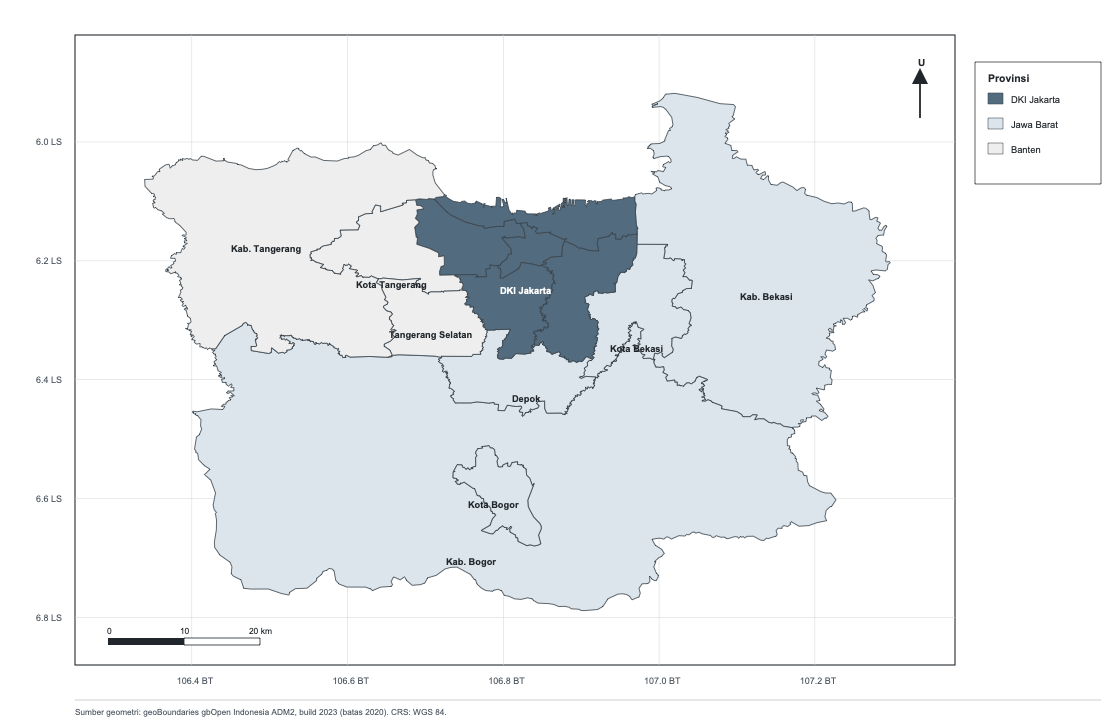
\includegraphics[width=0.98\textwidth]{bab4_admin.png}
  \caption{Batas administratif wilayah penelitian. Sumber: geoBoundaries gbOpen Indonesia ADM2, build 2023 dengan geometri yang merepresentasikan batas administratif tahun 2020; diunduh 19 September 2026. Proyeksi visual WGS84 geografis. Skala dan orientasi digunakan untuk pembacaan konteks.}
  \label{fig:bab4-admin}
\end{figure}

Gambar \ref{fig:bab4-admin} memperlihatkan posisi relatif sembilan unit dan menjadi peta batas tetap untuk pelaporan. Hubungan ekonomi, perjalanan, dan pelayanan dapat melintasi garis tersebut. Batas administrasi digunakan untuk menempatkan hasil pada kewenangan yang sesuai.

\begin{figure}[H]
  \centering
  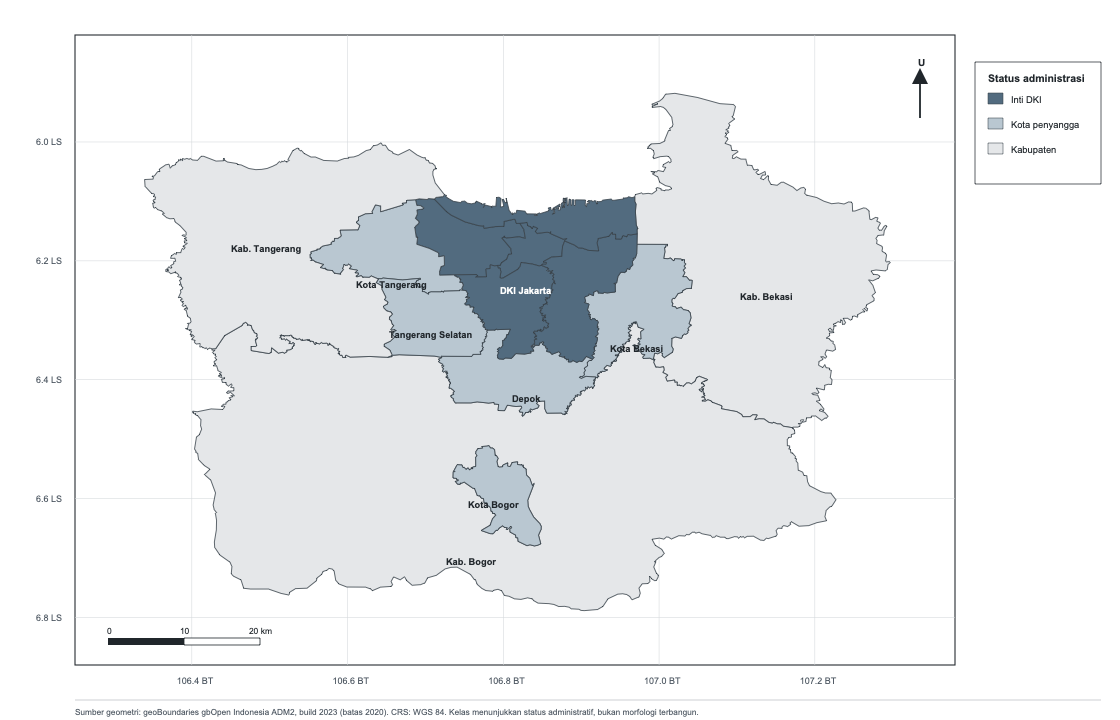
\includegraphics[width=0.98\textwidth]{bab4_status_administratif.png}
  \caption{Status administratif wilayah penelitian. Sumber geometri: geoBoundaries gbOpen Indonesia ADM2, build 2023 dengan batas tahun 2020. Kelas membedakan inti DKI, kota penyangga, dan kabupaten untuk kebutuhan pelaporan; kelas tersebut bukan ukuran morfologi terbangun atau kematangan pusat.}
  \label{fig:bab4-status-administratif}
\end{figure}

Gambar \ref{fig:bab4-status-administratif} membedakan status administrasi yang akan digunakan sebagai kondisi kontekstual. Kota dan kabupaten memiliki luas, kepadatan, kewenangan, serta komposisi wilayah yang berbeda. Perbedaan tersebut perlu diperiksa ketika hasil antarpusat dibandingkan, tetapi status kota tidak dengan sendirinya menetapkan suatu unit sebagai pusat sekunder.

\subsection{Cakupan wilayah dan aturan pembacaan}

Cakupan studi dipilih agar pusat inti dan wilayah penyangga utama dapat dibaca dalam satu kerangka. Kabupaten Bogor dan Kabupaten Bekasi berukuran luas dan memiliki kombinasi wilayah perkotaan, industri, serta perdesaan. Kabupaten Tangerang juga memuat koridor urban yang berbeda dari Kota Tangerang dan Kota Tangerang Selatan. Kota Bogor, Kota Depok, Kota Bekasi, Kota Tangerang, dan Kota Tangerang Selatan diperlakukan sebagai unit kota yang dapat memiliki massa lokal dan fungsi relatif sendiri.

Aturan pembacaannya adalah sebagai berikut. Pertama, angka penduduk dibaca sebagai massa lokal, bukan sebagai ukuran lengkap kapasitas pusat. Kedua, lokasi usaha, fasilitas, bangunan, jaringan, dan informasi operator diperlakukan sebagai sumber observasi yang dapat memiliki bias cakupan. Ketiga, hasil estimasi pekerjaan atau perjalanan tidak disamakan dengan pencatatan administratif. Keempat, peta kerja tidak dapat digunakan untuk menyimpulkan pusat sekunder sebelum indikator fungsi, integrasi, manfaat, dan beban diuji.

\section{Demografi dan massa lokal}

Massa lokal diperlukan sebagai tolok ukur ketika penelitian membandingkan fungsi pusat dengan ukuran wilayahnya. Untuk menjaga keterbandingan, Bab ini menggunakan proyeksi penduduk 2024 yang dipublikasikan BPS untuk unit di Jawa Barat dan Banten. Angka di bawah ditulis dalam ribu jiwa dan mengikuti definisi proyeksi pada publikasi asal. Perbedaan basis antara proyeksi, sensus, dan pencacahan administratif tetap dicatat sebagai sumber ketidakpastian.

\begin{table}[H]
\centering
\caption{Massa penduduk unit non-DKI dalam wilayah penelitian, 2024}
\label{tab:bab4-populasi}
\begin{tabularx}{\textwidth}{>{\raggedright\arraybackslash}p{0.38\textwidth} >{\raggedleft\arraybackslash}p{0.20\textwidth} >{\raggedright\arraybackslash}X}
\toprule
Unit administratif & Penduduk (ribu jiwa) & Sumber dan batas pembacaan \\
\midrule
Kabupaten Bogor & 5.682,30 & Proyeksi 2024 BPS Jawa Barat; kabupaten, bukan aglomerasi fungsional. \\
Kota Bogor & 1.078,35 & Proyeksi 2024 BPS Jawa Barat; kota administratif. \\
Kota Depok & 2.163,64 & Proyeksi 2024 BPS Jawa Barat; kota administratif. \\
Kabupaten Bekasi & 3.273,87 & Proyeksi 2024 BPS Jawa Barat; kabupaten. \\
Kota Bekasi & 2.644,06 & Proyeksi 2024 BPS Jawa Barat; kota administratif. \\
Kabupaten Tangerang & 3.400,49 & Proyeksi 2024 BPS Banten; kabupaten. \\
Kota Tangerang & 1.963,97 & Proyeksi 2024 BPS Banten; kota administratif. \\
Kota Tangerang Selatan & 1.399,50 & Proyeksi 2024 BPS Banten; kota administratif. \\
\bottomrule
\end{tabularx}
\smallskip
\parbox{\textwidth}{\footnotesize Catatan: angka Jawa Barat diambil dari tabel perbandingan kabupaten/kota pada \emph{Kota Depok Dalam Angka 2025}; angka Banten diambil dari tabel perbandingan kabupaten/kota pada \emph{Kota Tangerang Dalam Angka 2024}. Satuan, tahun, dan cakupan mengikuti sumber masing-masing \parencite{bpsjabar2025,bpsbanten2024}. Angka DKI tidak dijumlahkan ulang di tabel ini karena publikasi DKI memecahnya pada kota administrasi dan menggunakan tabel sektoral yang berbeda; rujukan auditnya adalah \emph{Provinsi DKI Jakarta Dalam Angka 2025} \parencite{bpsdki2025}.}
\end{table}

Tabel \ref{tab:bab4-populasi} menunjukkan massa lokal yang besar di beberapa wilayah luar DKI, terutama Kabupaten Bogor, Kabupaten Tangerang, Kabupaten Bekasi, Kota Bekasi, dan Kota Depok. Angka tersebut belum menunjukkan bahwa unit-unit itu memiliki fungsi metropolitan yang setara dengan Jakarta. Dalam analisis berikutnya, jumlah penduduk menjadi pembagi awal untuk menilai apakah fungsi yang teramati atau diperkirakan sebanding dengan massa lokalnya.

Perbedaan massa lokal juga penting bagi interpretasi hasil. Pusat dengan penduduk besar dapat memiliki fungsi yang tampak tinggi secara absolut tetapi biasa saja setelah dibandingkan dengan ukurannya. Sebaliknya, pusat dengan penduduk lebih kecil dapat menunjukkan fungsi khusus atau akses ke jaringan metropolitan tanpa memiliki jumlah fasilitas terbesar. Perbandingan relatif pada Bab 5 karena itu akan menggunakan indikator dengan unit dan tahun yang dijelaskan, serta menyertakan pemeriksaan sensitivitas terhadap pilihan pembagi.

\section{Morfologi terbangun dan jaringan transportasi}

Morfologi Jabodetabek terbentuk dari gabungan inti perkotaan padat, koridor jalan dan rel, kawasan industri, perumahan berskala besar, serta ruang terbuka yang tersisa di antara kawasan terbangun. Bentuk tersebut berubah melalui perluasan kawasan industri dan perumahan, pembangunan jalan tol dan jalan arteri, penguatan jaringan rel, serta pertumbuhan pusat perdagangan dan jasa. Studi tentang dekonsentrasi manufaktur dan transformasi pascasuburban menunjukkan bahwa perkembangan tersebut berlangsung tidak seragam antarwilayah \parencite{hudalahetal2013,hudalahfirman2012}.

Peta morfologi baru disusun setelah jejak bangunan atau raster tutupan terbangun lolos audit tahun, resolusi, klasifikasi, lisensi, dan cakupan. Naskah ini tidak memakai kelas administratif pada Gambar \ref{fig:bab4-status-administratif} sebagai pengganti morfologi. Jika lapisan yang lolos audit hanya tersedia untuk satu periode, hasilnya menjadi potret morfologi pada periode tersebut. Perubahan hanya dihitung apabila produk dan definisinya dapat disejajarkan.

Jaringan transportasi memberi jalur yang memungkinkan hubungan metropolitan terbentuk, tetapi keberadaan jaringan tidak sama dengan penggunaan. Laporan JUTPI 3 membahas jaringan publik masa depan dengan horizon 2045 dan menampilkan MRT, LRT, KCI, BRT, dan trem dalam peta usulan \parencite{jica2025jutpi}. Peta itu berguna untuk membaca arah kebijakan dan kemungkinan konektivitas, sedangkan analisis penelitian memerlukan pembedaan antara jaringan yang sudah beroperasi, jaringan yang direncanakan, frekuensi layanan, kapasitas, dan arus penumpang.

\begin{figure}[H]
  \centering
  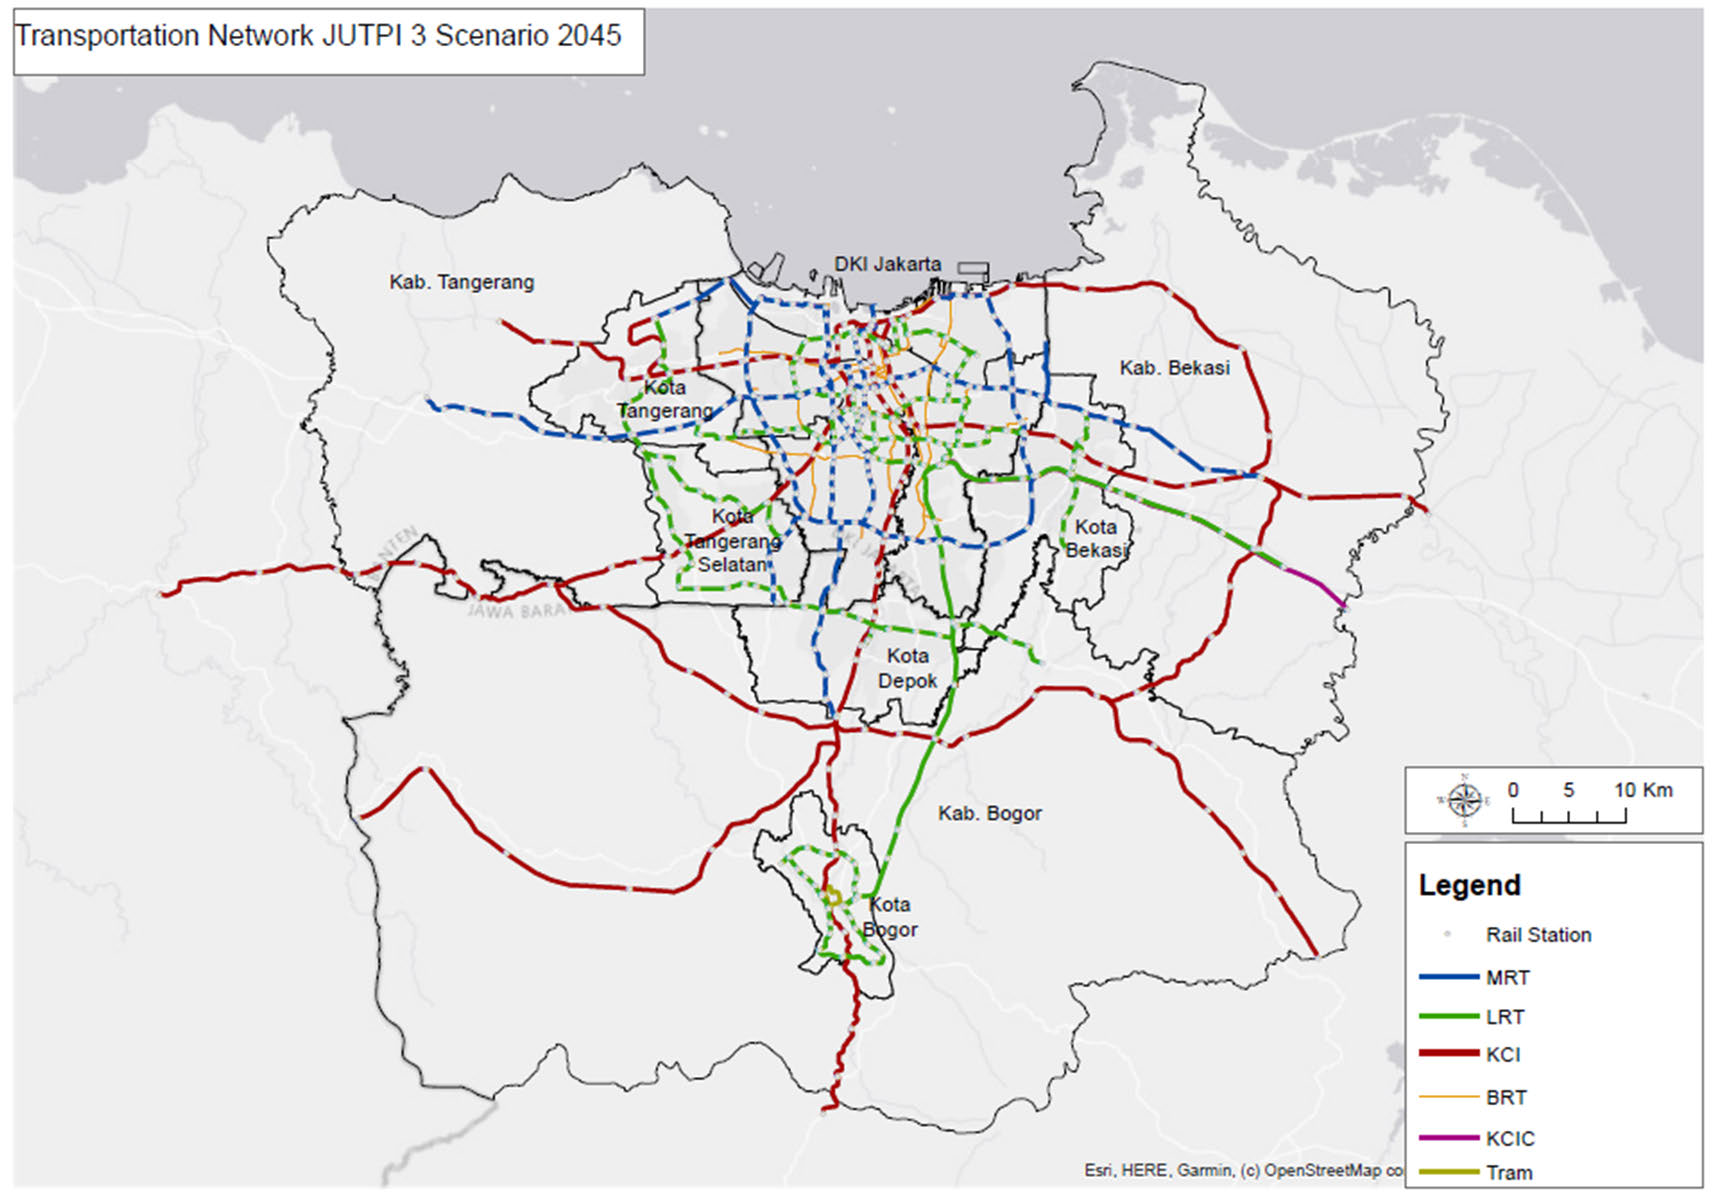
\includegraphics[width=0.90\textwidth]{bab4_network_jutpi.png}
  \caption{Peta jaringan angkutan umum masa depan yang diusulkan JUTPI 3 untuk Jabodetabek. Sumber: JICA Expert Team dalam \emph{Project Completion Report} 2025. Peta dibaca sebagai skenario kebijakan dan konteks jaringan, bukan pengamatan arus perjalanan aktual.}
  \label{fig:bab4-network}
\end{figure}

Peta jaringan JUTPI 3 memperlihatkan mengapa integrasi metropolitan tidak tepat direduksi menjadi kedekatan geometris. Hubungan antarwilayah dibentuk oleh simpul, koridor, waktu tempuh, kapasitas, pertukaran moda, dan hambatan perjalanan. Variabel jaringan aktual pada Bab 5 dipilih setelah audit terhadap data operator dan sumber terbuka. Rekaman CCTV yang tersedia dapat diolah dengan deteksi YOLO, pelacakan objek, dan garis hitung untuk mengestimasi arus pada titik serta waktu tertentu. SUMO digunakan hanya jika jaringan, permintaan, dan data kalibrasinya memadai.

\section{Industri, pusat pelayanan, dan aktivitas ekonomi}

Kawasan industri di Bekasi, Tangerang, dan sebagian Bogor merupakan konteks penting untuk membaca kemungkinan perubahan hubungan pekerjaan dan perjalanan. Penelitian sebelumnya mendokumentasikan perpindahan sebagian kegiatan manufaktur dari inti Jakarta ke kawasan metropolitan dan munculnya pola kerja antarsuburban \parencite{hudalahetal2013,permatasarihudalah2013,sadewoetal2023}. Namun, keberadaan kawasan industri tidak menunjukkan jumlah pekerjaan yang sedang tersedia pada tahun tertentu. Luas lahan, daftar perusahaan, lokasi gerbang, dan informasi operator harus dibedakan dari pekerjaan aktual.

Pusat pelayanan juga memiliki beberapa tingkat. Rumah sakit rujukan, kampus, pusat perdagangan, kantor pemerintahan, ruang budaya, dan fasilitas rekreasi dapat melayani penduduk lokal atau menarik pengguna dari wilayah lain. Lokasi fasilitas dari situs pemerintah, OpenStreetMap, dan direktori usaha dapat dipakai untuk membentuk observasi titik. Atribut seperti kapasitas, tingkat layanan, jam operasi, dan status aktif harus dicatat jika tersedia. Ketika atribut tidak tersedia, titik hanya dibaca sebagai indikasi keberadaan, bukan ukuran kualitas atau volume pengguna.

Sumber lokasi usaha seperti Google Maps, OpenStreetMap, data pemerintah daerah, dan situs operator dapat saling melengkapi. Setiap sumber memiliki mekanisme cakupan, pembaruan, dan duplikasi yang berbeda. Prosedur deduplikasi, pemeriksaan sampel manual, geocoding, dan pencatatan tanggal akses menjadi bagian dari audit. Keluaran akhirnya membedakan tiga status: observasi yang langsung terlihat pada sumber, estimasi yang dihitung dari observasi dengan asumsi, dan simulasi yang menggambarkan skenario.

\section{Kandidat pusat sekunder dan hubungan transportasi}

Penelitian tidak menetapkan pusat sekunder hanya karena sebuah wilayah berstatus kota atau memiliki penduduk besar. Label kerja digunakan untuk memeriksa beberapa lokasi yang secara awal memiliki kombinasi massa lokal, aktivitas, jaringan, dan potensi fungsi relatif. Label tersebut dapat berubah setelah data dibersihkan dan indikator diuji.

\begin{figure}[H]
  \centering
  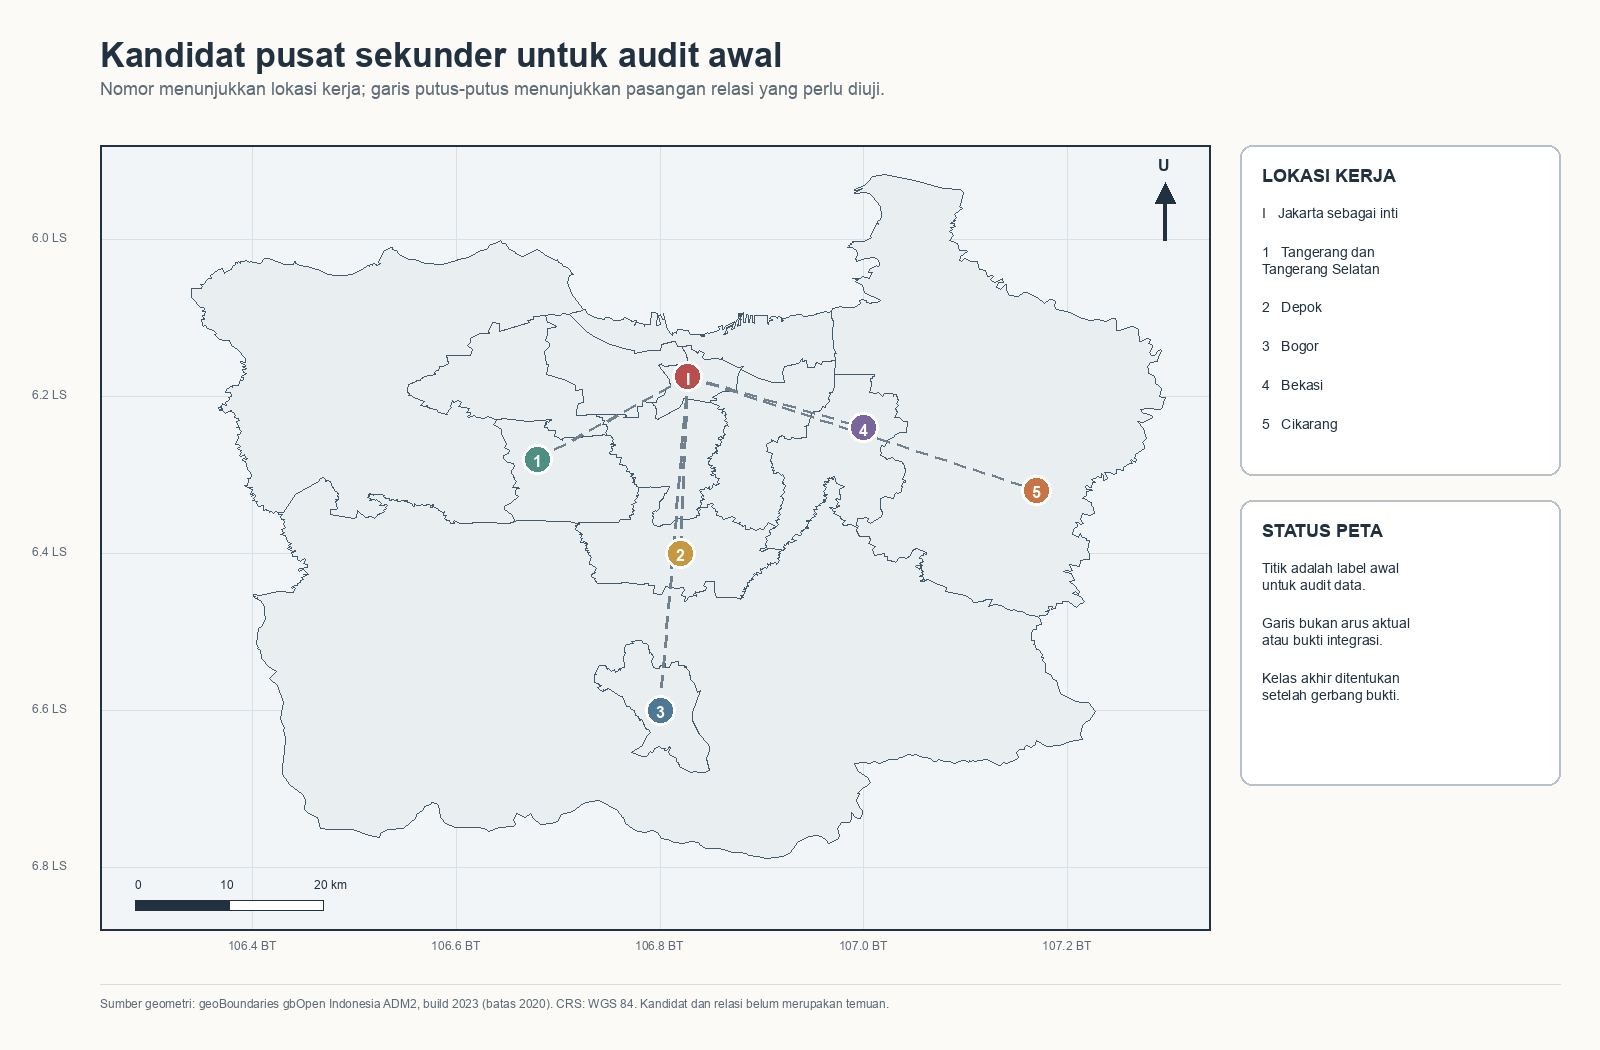
\includegraphics[width=0.98\textwidth]{bab4_candidates.png}
  \caption{Kandidat pusat sekunder sebagai label operasional awal. Nomor menunjukkan lokasi kerja dan garis putus-putus menunjukkan pasangan relasi yang perlu diaudit, bukan hasil klasifikasi atau arus perjalanan aktual. Sumber geometri: geoBoundaries gbOpen Indonesia ADM2; proyeksi visual WGS84 geografis dengan skala dan orientasi.}
  \label{fig:bab4-candidates}
\end{figure}

Gambar \ref{fig:bab4-candidates} menempatkan Jakarta inti, Tangerang dan Tangerang Selatan, Depok, Bogor, Bekasi, serta Cikarang sebagai titik audit awal. Cikarang berada dalam Kabupaten Bekasi dan dipisahkan sebagai lokasi kerja karena konteks industri dan jaringan dapat berbeda dari rata-rata kabupaten. Pemisahan tersebut belum berarti bahwa Cikarang akan menjadi pusat sekunder dalam hasil akhir. Unit analisis dapat berupa kota, kabupaten, koridor, atau klaster titik jika bukti dan tujuan pengukuran mengharuskannya.

Hubungan transportasi dan komuter dipakai untuk membaca hubungan fungsional. Survei Komuter Jabodetabek 2023 dari BPS menjadi rujukan terbuka untuk definisi dan tabulasi komuter, sementara laporan operator, berita resmi, dan data jaringan dapat digunakan untuk memeriksa layanan pada periode lain. Data perjalanan aktual tidak disimpulkan dari peta rencana. Jika data asal-tujuan terbuka tersedia, arus tersebut dilaporkan sebagai observasi. Jika hanya kapasitas armada, frekuensi, atau jumlah perjalanan yang tersedia, informasi tersebut digunakan sebagai batas atas, indikator kapasitas, atau bahan estimasi dengan asumsi yang ditulis.

Penggunaan CCTV dan SUMO ditempatkan sebagai penguatan bersyarat. Hitungan dari rekaman CCTV harus diuji pada sampel manual yang mewakili perbedaan kamera, kepadatan, cuaca, pencahayaan, sudut pandang, dan oklusi. Hasilnya dilaporkan sebagai estimasi menurut kamera, waktu, arah, dan kelas objek. Hitungan tersebut bukan matriks asal dan tujuan. SUMO dapat digunakan untuk simulasi skenario ketika jaringan, permintaan, dan parameter kalibrasi tersedia. Hasil simulasi tidak disebut arus aktual dan tidak menggantikan observasi.

\section{Audit sumber dan periode}

Audit sumber pada Tabel \ref{tab:bab4-audit} menjadi penghubung antara gambaran lokasi dan metode pengukuran. Tahun pada tabel adalah tahun observasi, tahun proyeksi, tahun geometri, atau tahun publikasi sesuai keterangan. Satu baris tidak boleh dipakai untuk menyiratkan seri waktu yang tidak ada.

\begingroup
\footnotesize
\setlength{\tabcolsep}{4pt}
\begin{longtable}{>{\raggedright\arraybackslash}p{0.19\textwidth} >{\raggedright\arraybackslash}p{0.17\textwidth} >{\raggedright\arraybackslash}p{0.15\textwidth} >{\raggedright\arraybackslash}p{0.41\textwidth}}
\caption{Audit sumber terbuka dan periode untuk Bab 4}\label{tab:bab4-audit}\\
\toprule
Konstruk/lapisan & Sumber & Tahun/periode & Status bukti dan batas penggunaan \\
\midrule
\endfirsthead
\caption[]{Audit sumber terbuka dan periode untuk Bab 4 (lanjutan)}\\
\toprule
Konstruk/lapisan & Sumber & Tahun/periode & Status bukti dan batas penggunaan \\
\midrule
\endhead
\midrule
\multicolumn{4}{r}{\footnotesize Dilanjutkan pada halaman berikutnya}\\
\endfoot
\bottomrule
\endlastfoot
Batas administratif & geoBoundaries gbOpen ADM2 & build 2023; geometri 2020 & Observasi geometri konteks. Tidak menetapkan batas fungsional atau daerah tangkapan \parencite{geoboundaries2023}. \\
Massa penduduk Jawa Barat & BPS, tabel kabupaten/kota dalam \emph{Kota Depok Dalam Angka 2025} & Proyeksi 2021--2025; digunakan 2024 & Angka proyeksi dalam ribu jiwa; unit kabupaten/kota. \\
Massa penduduk Banten & BPS, tabel kabupaten/kota dalam \emph{Kota Tangerang Dalam Angka 2024} & Proyeksi 2020--2024; digunakan 2024 & Angka proyeksi dalam ribu jiwa; unit kabupaten/kota. \\
Statistik DKI & BPS Provinsi DKI Jakarta, \emph{Provinsi DKI Jakarta Dalam Angka 2025} & Publikasi 2025; indikator sektoral bervariasi & Sumber audit untuk kota administrasi, demografi, ekonomi, dan layanan; angka dipakai bersama tahun indikator. \\
Jaringan dan skenario transportasi & JICA Expert Team, JUTPI 3 & Laporan 2025; jaringan usulan 2045 & Skenario dan konteks kebijakan. Tidak dibaca sebagai jaringan aktual atau arus aktual \parencite{jica2025jutpi}. \\
Komuter & BPS, Survei Komuter Jabodetabek & 2023 & Definisi dan tabulasi komuter. Cakupan, unit, dan tabel yang dipakai dicatat kembali pada manifest data. \\
Bangunan dan tutupan terbangun & sumber raster atau jejak bangunan terbuka yang lolos audit & periode mengikuti produk & Akan dipakai hanya jika tahun, resolusi, lisensi, dan metode ekstraksi dapat ditelusuri. \\
Lokasi usaha dan fasilitas & pemerintah daerah, OpenStreetMap, direktori usaha, dan situs operator & tanggal akses per ekstraksi & Observasi titik dengan bias cakupan. Deduplikasi dan pemeriksaan sampel wajib dicatat. \\
Rekaman lalu lintas titik & Rekaman CCTV yang telah tersedia & Periode mengikuti metadata setiap rekaman; belum diaudit & Video merupakan observasi mentah. Hitungan YOLO dan pelacakan objek berstatus estimasi turunan serta memerlukan validasi manual menurut kamera, waktu, arah, dan kelas objek. \\
Kandidat pusat & gabungan lapisan terbuka dan literatur & label awal Bab 4 & Status operasional; bukan hasil klasifikasi dan tidak menjadi bukti tunggal fungsi. \\
\end{longtable}
\endgroup

Tabel tersebut sengaja memisahkan sumber yang sudah memiliki angka dari sumber yang baru menjadi rujukan konteks. Peta JUTPI 3, misalnya, dapat memperlihatkan arah jaringan dan lokasi simpul yang direncanakan, tetapi tidak dapat dipakai untuk menghitung integrasi aktual tanpa data operasi. Demikian pula, direktori usaha dapat membantu menemukan lokasi dan perubahan keberadaan, tetapi tidak langsung mengukur omzet, jumlah pekerja, atau jumlah pengunjung.

\section{Batas interpretasi gambaran lokasi}

Bab 4 menyediakan batas administratif tetap untuk pemetaan antarsumber, gambaran massa lokal dan struktur wilayah untuk membaca perbedaan antarpusat, serta daftar titik dan lapisan terbuka yang akan diaudit dan diuji sensitivitasnya. Ketiganya menjadi konteks bagi pengukuran, bukan hasil diagnosis.

Bab ini tidak mengklaim bahwa semua indikator sudah memiliki rentang tahun yang sama. Seri waktu hanya dibentuk untuk indikator yang memiliki definisi, unit, dan cakupan yang dapat disejajarkan. Indikator dengan satu tahun atau periode berbeda tetap dapat digunakan sebagai konteks atau potret, dengan statusnya ditulis. Jika audit berikutnya menemukan bahwa satu sumber tidak cukup stabil, indikator tersebut diturunkan menjadi hasil estimasi atau dikeluarkan dari konstruksi inti tanpa mengubah arah penelitian.

Dengan aturan ini, istilah pusat sekunder berarti kandidat unit yang akan diuji terhadap fungsi relatif, integrasi, manfaat, beban, dan hubungan metropolitan. Istilah tersebut belum merupakan kesimpulan. Bab 5 menjadi tempat untuk menunjukkan apakah pola yang terukur lebih dekat dengan manfaat yang dipinjam, bayangan aglomerasi, campuran keduanya, atau hasil yang belum terselesaikan pada konstruk tertentu.

\printbibliography[heading=bibintoc,title={Daftar Pustaka}]
\end{document}
